%% abtex2-modelo-trabalho-academico.tex, v-1.9.2 laurocesar
%% Copyright 2012-2014 by abnTeX2 group at http://abntex2.googlecode.com/ 
%%
%% This work may be distributed and/or modified under the
%% conditions of the LaTeX Project Public License, either version 1.3
%% of this license or (at your option) any later version.
%% The latest version of this license is in
%%   http://www.latex-project.org/lppl.txt
%% and version 1.3 or later is part of all distributions of LaTeX
%% version 2005/12/01 or later.
%%
%% This work has the LPPL maintenance status `maintained'.
%% 
%% The Current Maintainer of this work is the abnTeX2 team, led
%% by Lauro César Araujo. Further information are available on 
%% http://abntex2.googlecode.com/
%%
%% This work consists of the files abntex2-modelo-trabalho-academico.tex,
%% abntex2-modelo-include-comandos and abntex2-modelo-references.bib
%%

% ------------------------------------------------------------------------
% ------------------------------------------------------------------------
% abnTeX2: Modelo de Trabalho Academico (tese de doutorado, dissertacao de
% mestrado e trabalhos monograficos em geral) em conformidade com 
% ABNT NBR 14724:2011: Informacao e documentacao - Trabalhos academicos -
% Apresentacao
% ------------------------------------------------------------------------
% ------------------------------------------------------------------------

%-------------------------------------------------------------------------
% Modelo adaptado especificamente para o contexto do PPgSI-EACH-USP por 
% Marcelo Fantinato, com auxílio dos Professores Norton T. Roman, Helton
% H. Bíscaro e Sarajane M. Peres, em 2015, com muitos agradecimentos aos 
% criadores da classe e do modelo base.
%
% 20/06/2017: inclusão de "lista de quadros" com base no especificado em:
% https://github.com/abntex/abntex2/wiki/HowToCriarNovoAmbienteListing,
% de autoria de "Eduardo de Santana Medeiros Alexandre".
%
%-------------------------------------------------------------------------

\documentclass[
	% -- opções da classe memoir --
	12pt,				% tamanho da fonte
	% openright,			% capítulos começam em pág ímpar (insere página vazia caso preciso)
	oneside,			% para impressão apenas no anverso (apenas frente). Oposto a twoside
	a4paper,			% tamanho do papel. 
	% -- opções da classe abntex2 --
	%chapter=TITLE,		% títulos de capítulos convertidos em letras maiúsculas
	%section=TITLE,		% títulos de seções convertidos em letras maiúsculas
	%subsection=TITLE,	% títulos de subseções convertidos em letras maiúsculas
	%subsubsection=TITLE,% títulos de subsubseções convertidos em letras maiúsculas
	% -- opções do pacote babel --
	english,			% idioma adicional para hifenização
	%french,				% idioma adicional para hifenização
	%spanish,			% idioma adicional para hifenização
	brazil				% o último idioma é o principal do documento
	]{abntex2ppgsi}

% ---
% Pacotes básicos 
% ---
% \usepackage{lmodern}			% Usa a fonte Latin Modern			
% \usepackage[T1]{fontenc}		% Selecao de codigos de fonte.
\usepackage[utf8]{inputenc}		% Codificacao do documento (conversão automática dos acentos)
\usepackage{lastpage}			% Usado pela Ficha catalográfica
\usepackage{indentfirst}		% Indenta o primeiro parágrafo de cada seção.
\usepackage{color}				% Controle das cores
\usepackage{graphicx}			% Inclusão de gráficos
\usepackage{microtype} 			% para melhorias de justificação
\usepackage{pdfpages}     %para incluir pdf
\usepackage{algorithm}			%para ilustrações do tipo algoritmo
\usepackage{mdwlist}			%para itens com espaço padrão da abnt
\usepackage[noend]{algpseudocode}			%para ilustrações do tipo algoritmo
		
% ---
% Pacotes adicionais, usados apenas no âmbito do Modelo Canônico do abnteX2
% ---
\usepackage{lipsum}				% para geração de dummy text
% ---

% ---
% Pacotes de citações
% ---
\usepackage[brazilian,hyperpageref]{backref}	 % Paginas com as citações na bibl
\usepackage[alf,abnt-etal-list=0,abnt-etal-text=it]{abntex2cite}	% Citações padrão ABNT

% --- 
% CONFIGURAÇÕES DE PACOTES
% --- 

% ---
% Configurações do pacote backref
% Usado sem a opção hyperpageref de backref
\renewcommand{\backrefpagesname}{Citado na(s) página(s):~}
% Texto padrão antes do número das páginas
\renewcommand{\backref}{}
% Define os textos da citação
\renewcommand*{\backrefalt}[4]{
	\ifcase #1 %
		Nenhuma citação no texto.%
	\or
		Citado na página #2.%
	\else
		Citado #1 vezes nas páginas #2.%
	\fi}%
% ---

% ---
% Informações de dados para CAPA e FOLHA DE ROSTO
% ---

%-------------------------------------------------------------------------
% Comentário adicional do PPgSI - Informações sobre o ``instituicao'':
%
% Não mexer. Deixar exatamente como está.
%
%-------------------------------------------------------------------------
\instituicao{
	UNIVERSIDADE DE SÃO PAULO
	\par
	ESCOLA DE ARTES, CIÊNCIAS E HUMANIDADES
	\par
	PROGRAMA DE PÓS-GRADUAÇÃO EM SISTEMAS DE INFORMAÇÃO}

%-------------------------------------------------------------------------
% Comentário adicional do PPgSI - Informações sobre o ``título'':
%
% Em maiúscula apenas a primeira letra da sentença (do título), exceto 
% nomes próprios, geográficos, institucionais ou Programas ou Projetos ou 
% siglas, os quais podem ter letras em maiúscula também.
%
% O subtítulo do trabalho é opcional.
% Sem ponto final.
%
% Atenção: o título da Dissertação na versão corrigida não pode mudar. 
% Ele deve ser idêntico ao da versão original.
%
%-------------------------------------------------------------------------
\titulo{A Importância da Acessibilidade Digital nas Aplicações Móveis: Um Estudo sobre os Comentários de Usuários no Google Play Store}

%-------------------------------------------------------------------------
% Comentário adicional do PPgSI - Informações sobre o ``autor'':
%
% Todas as letras em maiúsculas.
% Nome completo.
% Sem ponto final.
%-------------------------------------------------------------------------
\autor{\uppercase{Leandro Orlandin}}

%-------------------------------------------------------------------------
% Comentário adicional do PPgSI - Informações sobre o ``local'':
%
% Não incluir o ``estado''.
% Sem ponto final.
%-------------------------------------------------------------------------
\local{São Paulo}

%-------------------------------------------------------------------------
% Comentário adicional do PPgSI - Informações sobre a ``data'':
%
% Colocar o ano do depósito (ou seja, o ano da entrega) da respectiva 
% versão, seja ela a versão original (para a defesa) seja ela a versão 
% corrigida (depois da aprovação na defesa). 
%
% Atenção: Se a versão original for depositada no final do ano e a versão 
% corrigida for entregue no ano seguinte, o ano precisa ser atualizado no 
% caso da versão corrigida. 
% Cuidado, pois o ano da ``capa externa'' também precisa ser atualizado 
% nesse caso.
%
% Não incluir o dia, nem o mês.
% Sem ponto final.
%-------------------------------------------------------------------------
\data{2020}

%-------------------------------------------------------------------------
% Comentário adicional do PPgSI - Informações sobre o ``Orientador'':
%
% Se for uma professora, trocar por ``Profa. Dra.''
% Nome completo.
% Sem ponto final.
%-------------------------------------------------------------------------
\orientador{Prof. Dr. Orientador: Marcelo Medeiros Eler}

%-------------------------------------------------------------------------
% Comentário adicional do PPgSI - Informações sobre o ``Coorientador'':
%
% Opcional. Incluir apenas se houver co-orientador formal, de acordo com o 
% Regulamento do Programa.
%
% Se for uma professora, trocar por ``Profa. Dra.''
% Nome completo.
% Sem ponto final.
%-------------------------------------------------------------------------

%LORLANDIN - RETIRADO O COORIENTADOR
%\coorientador{Prof. Dr. Fulano de Tal}

\tipotrabalho{Dissertação (Mestrado)}

\preambulo{
%-------------------------------------------------------------------------
% Comentário adicional do PPgSI - Informações sobre o texto ``Versão 
% original'':
%
% Não usar para Qualificação.
% Não usar para versão corrigida de Dissertação.
%
%-------------------------------------------------------------------------
%LORLANDIN - RETIRADO POR SER QUALIFICAÇÃO
%Versão original \newline \newline \newline 
%-------------------------------------------------------------------------
% Comentário adicional do PPgSI - Informações sobre o ``texto principal do
% preambulo'':
%
% Para Qualificação, trocar por: Projeto de pesquisa para exame de qualificação apresentado à Escola de Artes, Ciências e Humanidades da Universidade de São Paulo como parte dos requisitos para obtenção do título de Mestre em Ciências pelo Programa de Pós-graduação em Sistemas de Informação.
%
%-------------------------------------------------------------------------
%LORLANDIN - SUBSTITUÍDO CONFORME ORIENTAÇÃO ACIMA - QUALIFICAÇÃO
Projeto de pesquisa para exame de qualificação apresentado à Escola de Artes, Ciências e Humanidades da Universidade de São Paulo como parte dos requisitos para obtenção do título de Mestre em Ciências pelo Programa de Pós-graduação em Sistemas de Informação.
%Dissertação apresentada à Escola de Artes, Ciências e Humanidades da Universidade de São Paulo para obtenção do título de Mestre em Ciências pelo Programa de Pós-graduação em Sistemas de Informação. 
%
\newline \newline Área de concentração: Metodologia e Técnicas da Computação
%-------------------------------------------------------------------------
% Comentário adicional do PPgSI - Informações sobre o texto da ``Versão 
% corrigida'':
%
% Não usar para Qualificação.
% Não usar para versão original de Dissertação.
% 
% Substituir ``xx de xxxxxxxxxxxxxxx de xxxx'' pela ``data da defesa''.
%
%-------------------------------------------------------------------------
%LORLANDIN - RETIRADO POR SER QUALIFICAÇÃO
%\newline \newline \newline Versão corrigida contendo as alterações solicitadas pela comissão julgadora em xx de xxxxxxxxxxxxxxx de xxxx. A versão original encontra-se em acervo reservado na Biblioteca da EACH-USP e na Biblioteca Digital de Teses e Dissertações da USP (BDTD), de acordo com a Resolução CoPGr 6018, de 13 de outubro de 2011.}
% ---
}

% ---
% Configurações de aparência do PDF final

% alterando o aspecto da cor azul
\definecolor{blue}{RGB}{41,5,195}

% informações do PDF
\makeatletter
\hypersetup{
     	%pagebackref=true,
		pdftitle={\@title}, 
		pdfauthor={\@author},
    	pdfsubject={\imprimirpreambulo},
	    pdfcreator={LaTeX com abnTeX2 adaptado para o PPgSI-EACH-USP},
		pdfkeywords={abnt}{latex}{abntex}{abntex2}{qualificação de mestrado}{dissertação de mestrado}{ppgsi}, 
		colorlinks=true,       		% false: boxed links; true: colored links
    	linkcolor=black,          	% color of internal links
    	citecolor=black,        		% color of links to bibliography
    	filecolor=black,      		% color of file links
		urlcolor=black,
		bookmarksdepth=4
}
\makeatother
% --- 

% --- 
% Espaçamentos entre linhas e parágrafos 
% --- 

% O tamanho do parágrafo é dado por:
\setlength{\parindent}{1.25cm}

% Controle do espaçamento entre um parágrafo e outro:
\setlength{\parskip}{0cm}  % tente também \onelineskip
\renewcommand{\baselinestretch}{1.5}

% ---
% compila o indice
% ---
\makeindex
% ---

	% Controlar linhas orfas e viuvas
  \clubpenalty10000
  \widowpenalty10000
  \displaywidowpenalty10000

% ----
% Início do documento
% ----
\begin{document}

% Retira espaço extra obsoleto entre as frases.
\frenchspacing 

% ----------------------------------------------------------
% ELEMENTOS PRÉ-TEXTUAIS
% ----------------------------------------------------------
% \pretextual

% ---
% Capa
% ---
%-------------------------------------------------------------------------
% Comentário adicional do PPgSI - Informações sobre a ``capa'':
%
% Esta é a ``capa'' principal/oficial do trabalho, a ser impressa apenas 
% para os casos de encadernação simples (ou seja, em ``espiral'' com 
% plástico na frente).
% 
% Não imprimir esta ``capa'' quando houver ``capa dura'' ou ``capa brochura'' 
% em que estas mesmas informações já estão presentes nela.
%
%-------------------------------------------------------------------------
\imprimircapa
% ---

% ---
% Folha de rosto
% (o * indica que haverá a ficha bibliográfica)
% ---
\imprimirfolhaderosto*
% ---

% ---
% Inserir a autorização para reprodução e ficha bibliografica
% ---

%-------------------------------------------------------------------------
% Comentário adicional do PPgSI - Informações sobre o texto da 
% ``autorização para reprodução e ficha bibliografica'':
%
% Página a ser usada apenas para Dissertação (tanto na versão original 
% quanto na versão corrigida).
%
% Solicitar a ficha catalográfica na Biblioteca da EACH. 
% Duas versões devem ser solicitadas, em dois momentos distintos: uma vez 
% para a versão original, e depois outra atualizada para a versão 
% corrigida.
%
% Atenção: esta página de ``autorização para reprodução e ficha 
% catalográfica'' deve ser impressa obrigatoriamente no verso da folha de 
% rosto.
%
% Não usar esta página para Qualificação.
%
% Substitua o arquivo ``fig_ficha_catalografica.pdf'' abaixo referenciado 
% pelo PDF elaborado pela Biblioteca
%
%-------------------------------------------------------------------------
%LORLANDIN - RETIRADO POR SER QUALIFICAÇÃO
%\begin{fichacatalografica}
%    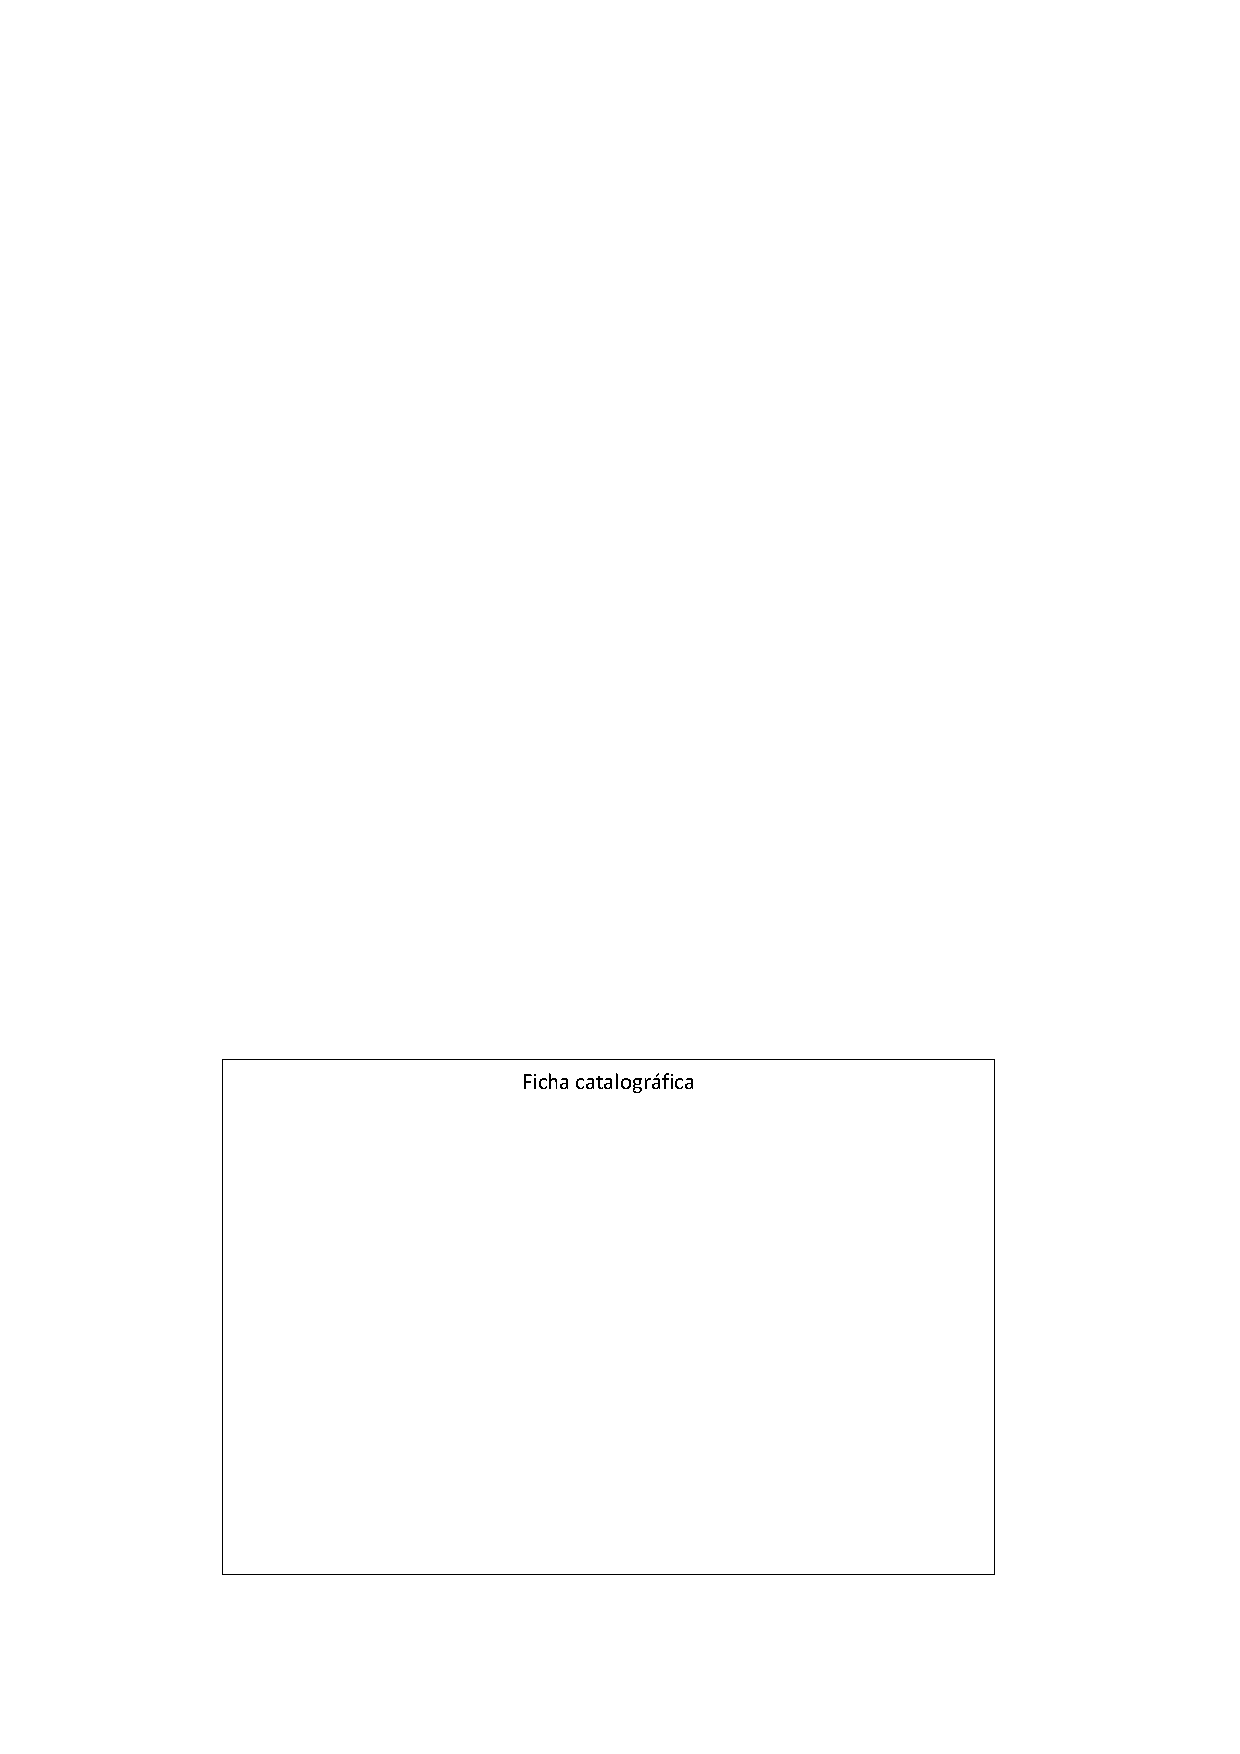
\includepdf{fig_ficha_catalografica.pdf}
%\end{fichacatalografica}



% ---
% Inserir errata
% ---
%-------------------------------------------------------------------------
% Comentário adicional do PPgSI - Informações sobre ``Errata'':
%
% Usar esta página de errata apenas em casos de excepcionais, e apenas 
% para a versão corrigida da Dissertação. Por exemplo, quando depois de
% já depositada e publicada a versão corrigida, ainda assim verifica-se
% a necessidade de alguma correção adicional.
%
% Se precisar usar esta página, busque a forma correta (o modelo correto) 
% para fazê-lo, de acordo com a norma ABNT.
%
% Não usar esta página para versão original de Dissertação.
% Não usar esta página para Qualificação.
%
%-------------------------------------------------------------------------
%LORLANDIN - RETIRADO POR SER QUALIFICAÇÃO
%\begin{errata}
%Elemento opcional para versão corrigida, depois de depositada.
%\end{errata}
% ---

% ---
% Inserir folha de aprovação
% ---

\begin{folhadeaprovacao}

%-------------------------------------------------------------------------
% Comentário adicional do PPgSI - Informações sobre ``Folha da aprovação'':
%
% Página a ser usada apenas para Dissertação.
%
% Não usar esta página para Qualificação.
%
% Substituir ``Fulano de Tal'' pelo nome completo do autor do trabalho, com 
% apenas as iniciais em maiúsculo.
%
% Substituir ``___ de ______________ de ______'' por: 
%     - Para versão original de Dissertação: deixar em branco, pois a data 
%       pode mudar, mesmo que ela já esteja prevista.
%     - Para versão corrigida de Dissertação: usar a data em que a defesa 
%       efetivamente ocorreu.
%
%-------------------------------------------------------------------------

%LORLANDIN - RETIRADO POR SER QUALIFICAÇÃO
%\noindent Dissertação de autoria de Fulano de Tal, sob o título \textbf{``\imprimirtitulo''}, apresentada à Escola de Artes, Ciências e Humanidades da Universidade de São Paulo, para obtenção do título de Mestre em Ciências pelo Programa de Pós-graduação em Sistemas de Informação, na área de concentração Metodologia e Técnicas da Computação, aprovada em \_\_\_\_\_\_\_ de \_\_\_\_\_\_\_\_\_\_\_\_\_\_\_\_\_\_\_\_\_\_ de \_\_\_\_\_\_\_\_\_\_ pela comissão julgadora constituída pelos doutores:

\vspace*{3cm}

\begin{center}
%-------------------------------------------------------------------------
% Comentário adicional do PPgSI - Informações sobre ``assinaturas'':
%
% Para versão original de Dissertação: deixar em 
% branco (ou seja, assim como está abaixo), pois os membros da banca podem
% mudar, mesmo que eles já estejam previstos.
% 
% Para versão corrigida de Dissertação: usar os dados dos examinadores que 
% efetivamente participaram da defesa. 
% 
% Para versão corrigida de Dissertação: em caso de ``professora'', trocar 
% por ``Profa. Dra.'' 
% 
% Para versão corrigida de Dissertação: ao colocar os nomes dos 
% examinadores, remover o sublinhado
% 
% Para versão corrigida de Dissertação: ao colocar os nomes dos 
% examinadores, usar seus nomes completos, exatamente conforme constam em 
% seus Currículos Lattes
% 
% Para versão corrigida de Dissertação: ao colocar os nomes das 
% instituições, remover o sublinhado e remover a palavra ``Instituição:''
%
% Para a versão corrigida de Dissertação: remova o texto “Instituição: ”, 
% ou seja, coloque apenas/diretamente o nome da instituição.
%
% Não abreviar os nomes das instituições.
%
%-------------------------------------------------------------------------
\_\_\_\_\_\_\_\_\_\_\_\_\_\_\_\_\_\_\_\_\_\_\_\_\_\_\_\_\_\_\_\_\_\_\_\_\_\_\_\_\_\_\_\_\_\_\_\_\_\_\_\_\_\_\_\_
\vspace*{0.2cm} 
\\ \textbf{Prof. Dr. \_\_\_\_\_\_\_\_\_\_\_\_\_\_\_\_\_\_\_\_\_\_\_\_\_\_\_\_\_\_\_\_\_\_\_\_\_\_\_\_\_\_\_\_\_\_\_\_\_\_\_\_\_\_\_\_\_\_\_\_\_\_} 
\\ \vspace*{0.2cm} 
Instituição: \_\_\_\_\_\_\_\_\_\_\_\_\_\_\_\_\_\_\_\_\_\_\_\_\_\_\_\_\_\_\_\_\_\_\_\_\_\_\_\_\_\_\_\_\_\_\_\_\_\_\_\_\_\_\_\_\_\_ 
\\ \vspace*{0.2cm}
Presidente 

\vspace*{2cm}

\_\_\_\_\_\_\_\_\_\_\_\_\_\_\_\_\_\_\_\_\_\_\_\_\_\_\_\_\_\_\_\_\_\_\_\_\_\_\_\_\_\_\_\_\_\_\_\_\_\_\_\_\_\_\_\_
\vspace*{0.2cm} 
\\ \textbf{Prof. Dr. \_\_\_\_\_\_\_\_\_\_\_\_\_\_\_\_\_\_\_\_\_\_\_\_\_\_\_\_\_\_\_\_\_\_\_\_\_\_\_\_\_\_\_\_\_\_\_\_\_\_\_\_\_\_\_\_\_\_\_\_\_\_} 
\\ \vspace*{0.2cm} 
Instituição: \_\_\_\_\_\_\_\_\_\_\_\_\_\_\_\_\_\_\_\_\_\_\_\_\_\_\_\_\_\_\_\_\_\_\_\_\_\_\_\_\_\_\_\_\_\_\_\_\_\_\_\_\_\_\_\_\_\_

\vspace*{2cm}

\_\_\_\_\_\_\_\_\_\_\_\_\_\_\_\_\_\_\_\_\_\_\_\_\_\_\_\_\_\_\_\_\_\_\_\_\_\_\_\_\_\_\_\_\_\_\_\_\_\_\_\_\_\_\_\_
\vspace*{0.2cm} 
\\ \textbf{Prof. Dr. \_\_\_\_\_\_\_\_\_\_\_\_\_\_\_\_\_\_\_\_\_\_\_\_\_\_\_\_\_\_\_\_\_\_\_\_\_\_\_\_\_\_\_\_\_\_\_\_\_\_\_\_\_\_\_\_\_\_\_\_\_\_} 
\\ \vspace*{0.2cm} 
Instituição: \_\_\_\_\_\_\_\_\_\_\_\_\_\_\_\_\_\_\_\_\_\_\_\_\_\_\_\_\_\_\_\_\_\_\_\_\_\_\_\_\_\_\_\_\_\_\_\_\_\_\_\_\_\_\_\_\_\_

\vspace*{2cm}

\_\_\_\_\_\_\_\_\_\_\_\_\_\_\_\_\_\_\_\_\_\_\_\_\_\_\_\_\_\_\_\_\_\_\_\_\_\_\_\_\_\_\_\_\_\_\_\_\_\_\_\_\_\_\_\_
\vspace*{0.2cm} 
\\ \textbf{Prof. Dr. \_\_\_\_\_\_\_\_\_\_\_\_\_\_\_\_\_\_\_\_\_\_\_\_\_\_\_\_\_\_\_\_\_\_\_\_\_\_\_\_\_\_\_\_\_\_\_\_\_\_\_\_\_\_\_\_\_\_\_\_\_\_} 
\\ \vspace*{0.2cm} 
Instituição: \_\_\_\_\_\_\_\_\_\_\_\_\_\_\_\_\_\_\_\_\_\_\_\_\_\_\_\_\_\_\_\_\_\_\_\_\_\_\_\_\_\_\_\_\_\_\_\_\_\_\_\_\_\_\_\_\_\_

\end{center}

\end{folhadeaprovacao}
% ---

% ---
% Dedicatória
% ---
%-------------------------------------------------------------------------
% Comentário adicional do PPgSI - Informações sobre ``Dedicatória'': 
%
% Opcional para Dissertação.
% Não sugerido para Qualificação.
% 
%-------------------------------------------------------------------------

%LORLANDIN - RETIRADO POR SER QUALIFICAÇÃO - REINSERIR PARA A DISSERTAÇÃO
%\begin{dedicatoria}
%   \vspace*{\fill}
%   \centering
%   \noindent
%   \textit{Escreva aqui sua dedicatória, se desejar, ou remova esta página...} 
%	 \vspace*{\fill}
%\end{dedicatoria}
% ---

% ---
% Agradecimentos
% ---
%-------------------------------------------------------------------------
% Comentário adicional do PPgSI - Informações sobre ``Agradecimentos'': 
%
% Opcional para Dissertação.
% Não sugerido para Qualificação.
% 
% 
% Financiamentos recebidos durante o projeto de mestrado, vindos de qualquer 
% agência de fomento, devem ser mencionados na seção de agradecimentos da dissertação. 
% Isso se aplica não apenas a bolsas de estudo, mas a qualquer tipo de financiamento, 
% tais como para apoio a participação em eventos, compra de materiais, traduções etc. 
% Especificamente para financiamento da Capes, siga as instruções contidas na portaria 
% 206, de 4/set/2018; para outras agências de fomento, procure as regras apropriadas.
%
% Portaria Capes 206, de 4/set/2018: 
% http://ppgsi.each.usp.br/arquivos/Portaria_0783227_Portaria_CAPES_DOU___206_de_2018.pdf 
%
%
%-------------------------------------------------------------------------

%LORLANDIN - RETIRADO POR SER QUALIFICAÇÃO
%\begin{agradecimentos}
%Texto de exemplo, texto de exemplo, texto de exemplo, texto de exemplo, texto de exemplo, texto de exemplo, texto de exemplo, texto de exemplo, texto de exemplo, texto de exemplo, texto de exemplo, texto de exemplo, texto de exemplo, texto de exemplo, texto de exemplo, texto de exemplo, texto de exemplo, texto de exemplo, texto de exemplo, texto de exemplo, texto de exemplo, texto de exemplo.

%Texto de exemplo, texto de exemplo, texto de exemplo, texto de exemplo, texto de exemplo, texto de exemplo, texto de exemplo, texto de exemplo, texto de exemplo, texto de exemplo, texto de exemplo, texto de exemplo, texto de exemplo, texto de exemplo, texto de exemplo, texto de exemplo, texto de exemplo, texto de exemplo, texto de exemplo, texto de exemplo, texto de exemplo, texto de exemplo.

%Texto de exemplo, texto de exemplo, texto de exemplo, texto de exemplo, texto de exemplo, texto de exemplo, texto de exemplo, texto de exemplo, texto de exemplo, texto de exemplo, texto de exemplo, texto de exemplo, texto de exemplo, texto de exemplo, texto de exemplo, texto de exemplo, texto de exemplo, texto de exemplo, texto de exemplo, texto de exemplo, texto de exemplo, texto de exemplo.

%Texto de exemplo, texto de exemplo, texto de exemplo, texto de exemplo, texto de exemplo, texto de exemplo, texto de exemplo, texto de exemplo, texto de exemplo, texto de exemplo, texto de exemplo, texto de exemplo, texto de exemplo, texto de exemplo, texto de exemplo, texto de exemplo, texto de exemplo, texto de exemplo, texto de exemplo, texto de exemplo, texto de exemplo, texto de exemplo.

%Texto de exemplo, texto de exemplo, texto de exemplo, texto de exemplo, texto de exemplo, texto de exemplo, texto de exemplo, texto de exemplo, texto de exemplo, texto de exemplo, texto de exemplo, texto de exemplo, texto de exemplo, texto de exemplo, texto de exemplo, texto de exemplo, texto de exemplo, texto de exemplo, texto de exemplo, texto de exemplo, texto de exemplo, texto de exemplo.
%\end{agradecimentos}
% ---

% ---
% Epígrafe
% ---
%-------------------------------------------------------------------------
% Comentário adicional do PPgSI - Informações sobre ``Epígrafe'': 
%
% Opcional para Dissertação.
% Não sugerido para Qualificação.
% 
%-------------------------------------------------------------------------
%LORLANDIN - RETIRADO POR SER QUALIFICAÇÃO
%\begin{epigrafe}
%    \vspace*{\fill}
%	\begin{flushright}
%		\textit{``Escreva aqui uma epígrafe, se desejar, ou remova esta página...''\\
%		(Autor da epígrafe)}
%	\end{flushright}
%\end{epigrafe}
% ---

% ---
% RESUMOS
% ---

% resumo em português
\setlength{\absparsep}{18pt} % ajusta o espaçamento dos parágrafos do resumo
%\begin{resumo}

%-------------------------------------------------------------------------
% Comentário adicional do PPgSI - Informações sobre ``referência'':
% 
% Troque os seguintes campos pelos dados de sua Dissertação (mantendo a 
% formatação e pontuação):
%   - SOBRENOME
%   - Nome1
%   - Nome2
%   - Nome3
%   - Título do trabalho: subtítulo do trabalho
%   - AnoDeDefesa
%
% Mantenha todas as demais informações exatamente como estão.
% 
% [Não usar essas informações de ``referência'' para Qualificação]
%
%-------------------------------------------------------------------------
%LORLANDIN - RETIRADO POR SER QUALIFICAÇÃO
%\begin{flushleft}
%SOBRENOME, Nome1 Nome2 Nome3. \textbf{Título do trabalho}: subtítulo do trabalho. \imprimirdata. \pageref{LastPage} f. Dissertação (Mestrado em Ciências) – Escola de Artes, Ciências e Humanidades, Universidade de São Paulo, São Paulo, AnoDeDefesa.
%\end{flushleft}

%Escreva aqui o texto do seu resumo... (redigido em parágrafo único, no máximo em uma página, contendo no ``máximo 500 palavras'', e apresentando um resumo de todos o seu trabalho, incluindo objetivos, metodologia, resultados e conclusões; não inclua apenas a contextualização até chegar nos objetivos, é importante fazer um resumo de todos os capítulos do texto, até chegar à conclusão). Texto de exemplo, texto de exemplo, texto de exemplo, texto de exemplo, texto de exemplo, texto de exemplo, texto de exemplo, texto de exemplo, texto de exemplo, texto de exemplo, texto de exemplo, texto de exemplo, texto de exemplo, texto de exemplo, texto de exemplo, texto de exemplo, texto de exemplo, texto de exemplo, texto de exemplo, texto de exemplo, texto de exemplo, texto de exemplo.

%Palavras-chaves: Palavra1. Palavra2. Palavra3. etc.
%\end{resumo}

% resumo em inglês
%-------------------------------------------------------------------------
% Comentário adicional do PPgSI - Informações sobre ``resumo em inglês''
% 
% Caso a Qualificação ou a Dissertação inteira seja elaborada no idioma inglês, 
% então o ``Abstract'' vem antes do ``Resumo''.
% 
%-------------------------------------------------------------------------
%LORLANDIN - RETIRADO POR SER QUALIFICAÇÃO
%\begin{resumo}[Abstract]
%\begin{otherlanguage*}{english}

%-------------------------------------------------------------------------
% Comentário adicional do PPgSI - Informações sobre ``referência em inglês''
% 
% Troque os seguintes campos pelos dados de sua Dissertação (mantendo a 
% formatação e pontuação):
%     - SURNAME
%     - FirstName1
%     - MiddleName1
%     - MiddleName2
%     - Work title: work subtitle
%     - DefenseYear (Ano de Defesa)
%
% Mantenha todas as demais informações exatamente como estão.
%
% [Não usar essas informações de ``referência'' para Qualificação]
%
%-------------------------------------------------------------------------
%LORLANDIN - RETIRADO POR SER QUALIFICAÇÃO
%\begin{flushleft}
%SURNAME, FirstName MiddleName1 MiddleName2. \textbf{Work title}: work subtitle. \imprimirdata. \pageref{LastPage} p. Dissertation (Master of Science) – School of Arts, Sciences and Humanities, University of São Paulo, São Paulo, DefenseYear. 
%\end{flushleft}

%Write here the English version of your ``Resumo''. Example text, example text, example text, example text, example text, example text, example text, example text, example text, example text, example text, example text, example text, example text, example text, example text, example text, example text, example text, example text, example text, example text, example text, example text, example text, example text, example text, example text, example text, example text, example text, example text, example text, example text, example text, example text, example text, example text, example text, example text, example text, example text, example text, example text, example text, example text, example text.

%LORLANDIN - RETIRADO POR SER QUALIFICAÇÃO
%Keywords: Keyword1. Keyword2. Keyword3. etc.
%\end{otherlanguage*}
%\end{resumo}

% ---
% ---
% inserir lista de figuras
% ---
\pdfbookmark[0]{\listfigurename}{lof}
\listoffigures*
\cleardoublepage
% ---

% ---
% inserir lista de algoritmos
% ---
\pdfbookmark[0]{\listalgorithmname}{loa}
\listofalgorithms
\cleardoublepage

% ---
% inserir lista de quadros
% ---
\pdfbookmark[0]{\listofquadrosname}{loq}
\listofquadros*
\cleardoublepage


% ---
% inserir lista de tabelas
% ---
\pdfbookmark[0]{\listtablename}{lot}
\listoftables*
\cleardoublepage
% ---

% ---
% inserir lista de abreviaturas e siglas
% ---
%-------------------------------------------------------------------------
% Comentário adicional do PPgSI - Informações sobre ``Lista de abreviaturas 
% e siglas'': 
%
% Opcional.
% Uma vez que se deseja usar, é necessário manter padrão e consistência no
% trabalho inteiro.
% Se usar: inserir em ordem alfabética.
%
%-------------------------------------------------------------------------
%LORLANDIN - RETIRADO POR SER QUALIFICAÇÃO
%\begin{siglas}
%  \item[Sigla/abreviatura 1] Definição da sigla ou da abreviatura por extenso
%  \item[Sigla/abreviatura 2] Definição da sigla ou da abreviatura por extenso
%  \item[Sigla/abreviatura 3] Definição da sigla ou da abreviatura por extenso
%  \item[Sigla/abreviatura 4] Definição da sigla ou da abreviatura por extenso
%  \item[Sigla/abreviatura 5] Definição da sigla ou da abreviatura por extenso
%  \item[Sigla/abreviatura 6] Definição da sigla ou da abreviatura por extenso
%  \item[Sigla/abreviatura 7] Definição da sigla ou da abreviatura por extenso
%  \item[Sigla/abreviatura 8] Definição da sigla ou da abreviatura por extenso
%  \item[Sigla/abreviatura 9] Definição da sigla ou da abreviatura por extenso
%  \item[Sigla/abreviatura 10] Definição da sigla ou da abreviatura por extenso
%\end{siglas}
% ---

% ---
% inserir lista de símbolos
% ---
%-------------------------------------------------------------------------
% Comentário adicional do PPgSI - Informações sobre ``Lista de símbolos'': 
%
% Opcional.
% Uma vez que se deseja usar, é necessário manter padrão e consistência no
% trabalho inteiro.
% Se usar: inserir na ordem em que aparece no texto.
% 
%-------------------------------------------------------------------------
\begin{simbolos}
  \item[$ \Gamma $] Letra grega Gama
  \item[$ \Lambda $] Lambda
  \item[$ \zeta $] Letra grega minúscula zeta
  \item[$ \in $] Pertence
\end{simbolos}
% ---

% ---
% inserir o sumario
% ---
\pdfbookmark[0]{\contentsname}{toc}
\tableofcontents*
\cleardoublepage
% ---



% ----------------------------------------------------------
% ELEMENTOS TEXTUAIS
% ----------------------------------------------------------
\textual



%-------------------------------------------------------------------------
% Comentário adicional do PPgSI - Informações sobre ``títulos de seções''
% 
% Para todos os títulos (seções, subseções, tabelas, ilustrações, etc.):
%
% Em maiúscula apenas a primeira letra da sentença (do título), exceto 
% nomes próprios, geográficos, institucionais ou Programas ou Projetos ou
% siglas, os quais podem ter letras em maiúscula também.
%
%-------------------------------------------------------------------------
\chapter{Introdução}



\section{Contextualização}

Uma importante parcela da população mundial possui algum tipo de deficiência. 
De acordo com a Organização Mundial da Saúde - OMS (\textit{World Health Organization - WHO})\footnote{http://documents.worldbank.org/curated/en/665131468331271288/Main-report}, 
as estimativas são de que este público seja superior a 1 bilhão de pessoas. Considerando a população brasileira, as estimativas do censo de 2010\footnote{https://biblioteca.ibge.gov.br/visualizacao/periodicos/94/cd\_2010\_religiao\_deficiencia.pdf} são de que aproximadamente 18,8\% apresenta algum tipo de deficiência visual, 5,1\% deficiência auditiva, 7\% deficiência motora e 1,4\% deficiência mental ou intelectual. É importante salientar também que esses percentuais se agravam para a população idosa.

As pessoas com deficiência enfrentam barreiras na execução das mais diversas atividades cotidianas, incluindo o uso de serviços e de produtos eletrônicos. 
Neste contexto, a acessibilidade digital tem o objetivo de remover as barreiras que possam impedir ou dificultar os usuários a perceber, entender e operar produtos digitais de forma completa, segura e autônoma~\cite{wcag,w3cwai}.
Embora a acessibilidade digital tenha impacto na usabilidade e na qualidade global de qualquer software~\cite{Gay2018,ISO25010}, ela tem o foco nas necessidades específicas de pessoas com deficiência~\cite{ISO9241:11}.


Muitos avanços foram realizados nesta área ao longo dos anos para promover a acessibilidade digital: a criação de tecnologia assistiva, como leitores de tela e navegação por voz; 
a criação de padrões e guias de acessibilidade para orientar a produção de conteúdo e aplicações acessíveis, como o WCAG (\textit{Web Content Accessibility Guideline}) do W3C (\textit{The World Wide Web Consortium});
a criação de ferramentas para o desenvolvimento e avaliação de acessibilidade~\cite{Silva2018survey};
e a publicação de diversas leis que tornam obrigatório o desenvolvimento de produtos digitais acessíveis na esfera pública e privada~\cite{Lazar2019}.
A acessibilidade digital teve o foco inicial nas páginas e aplicações \textit{web} dado que diversas organizações adotaram esta plataforma para a divulgação de informação e para a realização de negócios, mas o aumento do uso de \textit{smartphones} e de suas aplicações trouxe também o foco para a acessibilidade digital móvel.


%Paralelo a este cenário, identifica-se também um aumento considerável do número de softwares para dispositivos móveis\footnote{https://www.statista.com/statistics/266210/number-of-available-applications-in-the-google-play-store/} denominados como aplicações móveis (ou apenas \textit{apps}). Esta explosão de \textit{apps} disponíveis para serem instalados e utilizados em celulares, tablets ou até mesmo em computadores, passou de 30 mil em 2009 para mais de 3 milhões em 2018, evidenciando assim a importância dos mesmos em muitos aspectos de nossas atividades cotidianas \cite{storeanalysis}.

%A partir dos fatores acima, índices de deficiência da população e utilização dos dispositivos móveis no cotidiano, atesta-se a importância da acessibilidade digital neste novo panorama mundial, essa representando a capacidade do software de ser utilizado independentemente da condição física, mental ou intelectual do usuário \cite{w3cwai}. 


\section{Lacuna de Pesquisa}

Infelizmente, 
apesar da existência de recursos para o desenvolvimento de aplicações acessíveis, 
diversos estudos evidenciaram uma falta geral de acessibilidade em aplicações móveis de diversas categorias, tamanhos, complexidade e popularidade~\cite{serra2015accessibility,eler2018mate,Yan2019currentstatus,Vendome2019,Alshayban2020,AcostaVargas2020}.
O mesmo fenômeno tem sido observado em aplicações \textit{web}, e por isso diversos estudos foram conduzidos para entender as razões que explicam a falta de acessibilidade observada. A maioria desses estudos investigou a consciência, o conhecimento e as questões organizacionais que impactam o desenvolvimento de software acessível e constatou que a maioria dos desenvolvedores tem pouco conhecimento sobre acessibilidade, as demandas por manutenção e novos produtos de software são muito altas, os prazos são curtos, não há treinamento adequado e o tema acessibilidade não é uma prioridade das organizações~\cite{  
lazar2004improving,Freire2008survey,oliveira2017strategies,Inal2019,barzilai2008factors,Putnam:2012}. Um estudo recente realizado com mais de 870 desenvolvedores de aplicações móveis no Brasil mostrou um comportamento semelhante nesta plataforma específica.


Se por um lado o conhecimento dos desenvolvedores e o contexto organizacional não favorecem o desenvolvimento de aplicações acessíveis, um outro fator pode fazer a diferença neste cenário: as requisições dos usuários. 
No contexto do desenvolvimento e evolução de aplicações móveis, 
é comum que as organizações utilizem avaliações (notas e comentários) realizadas pelos usuários nas lojas de aplicativos para planejar a correção de defeitos e o lançamento de novas funcionalidades, pois isso geralmente resulta em melhores avaliações, o que pode dar destaque e potencializar a instalação por outros usuários~\cite{nayebi,Palomba2015userreviews,Palomba2018crowdsourcing,Li2018MobileAE,Ciurumelea2017analyzing,Ortega2015thesis}.

Considerando que os comentários e as notas recebidas nas avaliações dos usuários são utilizados para corrigir falhas e evoluir aplicações móveis, duas questões de pesquisa são destacadas neste trabalho:
\begin{itemize}
 \item Os usuários de aplicações móveis mencionam aspectos relacionados à acessibilidade em suas avaliações publicadas nas lojas de aplicativos?
 \item Os problemas de acessibilidade relatados nas avaliações dos usuários têm impacto na evolução das aplicações móveis?
\end{itemize}

Diversos estudos sobre avaliações dos usuários em lojas de aplicativos foram realizados para entender as demandas dos usuários e as respostas dos desenvolvedores e das organizações~\cite{Iacob2013retrieving,Pagano2013userfeedback,Iacob2014online,Mcilroy2016analyzing,Sorbo2017surf,Ciurumelea2017analyzing,Ortega2015thesis,Li2018MobileAE,Pelloni2018becloma,Panichella2015how}. Os trabalhos encontrados na literatura classificam as avaliações dos usuários de diferentes formas: 
relato de falha, reclamações em geral, requisição de nova funcionalidade, solução de propostas, problemas com o custo, incompatibilidades, dificuldades com a rede, preocupações com segurança e privacidade, consumo de memória e bateria, elogios, e questões relacionadas à interface com o usuário.
Apesar de alguns estudos classificarem avaliações relacionadas à interface com o usuário, nenhuma delas fez uma diferenciação ou um detalhamento sobre os aspectos de acessibilidade abordados pelos usuários, tampouco enfatizaram a evolução da acessibilidade das aplicações. 


\section{Objetivo} 

O objetivo geral deste projeto de pesquisa é investigar se as avaliações feitas por usuários abordam aspectos relacionados à acessibilidade do produto, e se essas avaliações têm algum efeito na melhoria da acessibilidade da aplicação. Mais especificamente, deseja-se saber:
\begin{itemize}
 \item A quantidade e a distribuição de avaliações relacionadas à acessibilidade da aplicação
 \item A diversidade de tipos de violações de acessibilidade mencionadas nas avaliações
 \item O impacto das questões de acessibilidade nas notas atribuídas pelos usuários
 \item A quantidade e a distribuição de modificações relacionadas à acessibilidade da aplicação realizadas no código-fonte
 %\item A evolução da quantidade de violações encontradas nas diferentes versões da aplicação
\end{itemize}



\section{Justificativa e relavância}

Como as avaliações dos usuários são uma importante ferramenta para direcionar a evolução e a melhoria de aplicações móveis, 
é importante entender se e como as avaliações publicadas em lojas de aplicativos estão sendo utilizadas para informar aos desenvolvedores e às organizações questões relacionadas à acessibilidade das aplicações avaliadas. 
Além disso, também é fundamental entender se as questões de acessibilidade abordadas pelos usuários são levadas em consideração na evolução das aplicações avaliadas. 

Desta forma, os resultados da investigação aqui proposta podem dar evidências de que as pessoas com deficiência deveriam manifestar explicitamente as barreiras que enfrentam para usar aplicações, e assim pressionar desenvolvedores e organizações a aperfeiçoarem seus produtos.
Adicionalmente, mostrar que os diversos tipos de violações de acessibilidade trazem problemas reais para usuários e podem motivar desenvolvedores a levar em consideração as recomendações dos padrões e guias de acessibilidade enquanto projetam as interfaces de suas aplicações.


\section{Metodologia}

%Desta forma, esta proposta de pesquisa visa realizar um estudo amplo e generalizado envolvendo o tema acessibilidade sobre os comentários dos usuários na loja de aplicativos móveis \textit{Google Play Store}, \textit{commits} e \textit{issues} cadastrados pelos desenvolvedores em repositório aberto de código fonte \textit{Github}.

%As justificativas que visam embasar esta investigação pretendem 
%i) identificar se existe um volume significativo de comentários envolvendo acessibilidade e sua distribuição de acordo com as categorias dos \textit{apps},
%ii) analisar a diversificação dos comentários de acordo com padrões internacionais de acessibilidade \cite{bbc} e
%iii) se existe um relacionamento entre a classificação do comentário de acordo com a acessibilidade e à respectiva nota dada ao aplicativo pelo próprio usuário.
%iv) a correlação quantitativa entre os comentários, commits e issues

%Com este estudo, será possível confirmar a existência de uma pressão dos usuários frente aos desenvolvedores e empresas de aplicativos no que diz respeito às funcionalidades envolvendo acessibilidade.

Os objetivos desta proposta de pesquisa serão alcançados por meio da execução das seguintes atividades: 
\begin{itemize}
 \item Seleção de um conjunto de aplicações móveis cujas avaliações publicadas na loja de aplicativos serão analisadas.
 \item Obtenção das avaliações (comentários e notas atribuídas) dos usuários das aplicações selecionadas.
 \item Obtenção das sugestões de modificações (correção de defeitos, melhorias, novas funcionalidades - \textit{issues}) e alterações (\textit{commits}) no código das aplicações selecionadas por meio do acesso a seus repositórios de código.
 \item Seleção das avaliações dos usuários, sugestões de modificações e alterações que abordam aspectos da acessibilidade das aplicações selecionadas.
 \item Análise das avaliações, sugestões de modificações e alterações relacionadas à acessibilidade das aplicações.
 \end{itemize}

A metodologia deste trabalho está detalhada no Capítulo~\ref{chap:proposta}, onde todas as decisões tomadas para a condução deste projeto de pesquisa são apresentadas e justificadas. 

%Será definido um conjunto de aplicações móveis, com a condição inicial de que possuam versões de suas instalações (arquivos de instalação com extensão \textit{apk}) disponíveis no repositório F-Droid\footnote{https://f-droid.org/}. Este requisito permitirá que a pesquisa seja posteriormente evoluída, através de comparações entre os problemas de acessibilidade encontrados em diferentes versões do software, fora do escopo deste projeto. É importante que o levantamento selecione aplicações de diferentes categorias, como por exemplo: navegação, finanças e leitura.

%Uma nova ferramenta, em linguagem Python, será implementada para coletar os comentários dos aplicativos e validar a existência de versões do software de instalação no repositório de F-Droid. Esta condição inicial de validação poderá ser excluída se por ventura o conjunto for restrito a determinadas categorias ou mesmo possuam reduzido número de comentários envolvendo acessibilidade.

%Com base no \textit{W3C} \cite{wcag} e no \textit{BBC Guidelines} \cite{bbc}, serão estabelecidas palavras-chave que, em existindo no comentário, indicarão a possibilidade do mesmo se referir a uma diretriz de acessibilidade.

%Em posse dos comentários e das palavras-chave, será possível iniciar um processo de averiguação manual se os mesmos abordam o tema acessibilidade e qual foi a mensagem transmitida pelo usuário (pedido de correção ou cumprimentos pelo aplicativo).

%A mesma metodologia aplicada para a obtenção e avaliação dos comentários será utilizada sobre os textos informativos dos desenvolvedores quando da realização dos \textit{commits} e cadastramento das \textit{issues} no repositório de código fonte aberto \textit{Github}.

%Em posse destes dados, será realizado então um estudo que visa identificar uma correlação quantitativa entre as 3 bases de informações: comentários, \textit{commits} e \textit{issues}.


%Com a intenção de endereçar este tema auxiliando os designers e desenvolvedores de software a criar produtos acessíveis, vários padrões têm sido propostos e amplamente utilizados, principalmente aqueles ligados ao \textit{World Wide Web Consortium - W3C} \cite{wcag} e ao \textit{BBC Guidelines} \cite{bbc}. No âmbito nacional destaca-se o Modelo de Acessibilidade em Governo Eletrônico, ou simplesmente eMAG \cite{emag}. Todavia, é possível observar em estudos que ainda existe uma falta de acessibilidade nas aplicações \cite{smartcities,Eler2018mate,Quispe2018accessibility,Serra2015accessibility,Yan2019currentstatus}.

%É fundamental que não apenas os requisitos funcionais sejam garantidos pelas aplicações, mas também a disponibilização das mesmas considerando sua acessibilidade \cite{Oliveira2017strategies}. No âmbito de \textit{apps}, tem-se como importante característica suas constantes atualizações através de novas versões nas lojas de aplicativos (e.g. \textit{Google Play Store}) \cite{nayebi,Palompa2018crowdsourcing}. Este processo de frequente revisão ao longo do tempo torna as aplicações mais maduras, com inclusão de novas funcionalidades e correções de erros.

%Em muitos estudos identifica-se que tanto as classificações quanto os comentários dos usuários nas lojas de aplicativos são um importante direcionador para os desenvolvedores no momento do lançamento de novas versões \cite{Ciurumelea2017analyzing,Li2018MobileAE,Ortega2015thesis,Palomba2015userreviews,Palompa2018crowdsourcing,Pelloni2018becloma}. Considerando assim que os comentários orientam o desenvolvimento das \textit{apps} e que mesmo as mais maduras e populares apresentam problemas de acessibilidade \cite{Eler2018mate}, as dúvidas que surgem é se os usuários reportam suas dificuldades referentes à acessibilidade nas lojas de aplicativos, e do quão relevante são estes comentários para os desenvolvedores.



%Diferentes taxonomias são empregadas nos estudos dos comentários \cite{Ciurumelea2017analyzing,Sorbo2017surf,Iacob2013retrieving,Iacob2014online,Li2018MobileAE,Mcilroy2016analyzing,Ortega2015thesis,Pagano2013userfeedback,Panichella2015how,Pelloni2018becloma}, e apesar de alguns destes trabalhos citarem inclusive interfaces com usuário, não se observa estudos que possuam detalhamento a respeito dos problemas relacionados à acessibilidade digital.





%falar bem rapidamente como chegaremos lá
%selecionaremos um conjunto de aplicações
%implementar ferramentas para coletar estes comentários
%analisaremos estes comentários
%definiremos palavras-chave
%validação manual
%utilizaremos PLN (mas precisamos definir para quê utilizar a mesma) se dividirmos quantos tópicos a pessoa fala em cada comentários seria interessante
%quando a pessoa apenas reclama de algo a nota é ruim, porém quando existem outros assuntos envolvidos e algum deles pode ser elogios, a nota pode ser melhor.....
%análise de sentimento para extrair algo



\section{Organização}

Esta proposta de pesquisa está organizada da seguinte forma:
no Capítulo~\ref{chap:background} são apresentados os conceitos fundamentais que embasam este projeto de pesquisa,
no Capítulo~\ref{chap:proposta} a metodologia deste projeto de pesquisa é apresentada em detalhes,
e no Capítulo~\ref{chap:atividades} as atividades já realizadas desta proposta de pesquisa são apresentadas.



\label{chap:introducao}

\chapter{Revisão de Literatura}
\label{chap:background}

Segundo o site \textit{Dicio - Dicionário Online de Português}, a definição de acessibilidade pode ser dada como sendo \textit{a propriedade de material confeccionado para que qualquer pessoa tenha acesso, consiga ver, usar, compreender, principalmente de material que se destina à inclusão social de pessoas com alguma deficiência} \footnote{https://www.dicio.com.br/acessibilidade/}. Trata-se da possibilidade e condição de qualquer indivíduo alcançar os elementos funcionais do ambiente construído, para assim permitir sua utilização \cite{camilamaster}.

Para o caso de acessibilidade digital, e conforme visto anteriormente, essa representa a capacidade de um software ser utilizado, independentemente da condição física, mental ou intelectual do usuário \cite{w3cwai}. Trata-se da flexibilidade do software em se adaptar às necessidades de cada usuário, suas preferências e limitações \cite{camilamaster}. Este fator torna-se mais importante no contexto mundial atual em decorrência dos índices de pessoas com algum tipo de deficiência e da alta demanda por \textit{apps} em dispositivos móveis \cite{storeanalysis}.

Normalmente a acessibilidade digital é associada exclusivamente às dificuldades motoras, físicas ou sensoriais dos indivíduos com necessidades especiais, sendo desconsiderada importante parcela da população, como por exemplo idosos ou crianças. Uma aplicação que não seja acessível a um indivíduo não pode ser considerada eficaz, eficiente ou agradável ao mesmo \cite{santarosa}.

\section{Padrões de Acessibilidade}
Para atender a estas necessidades, diversos padrões foram definidos, com destaque para o WCAG, BBC Guidelines e eMAG, utilizados nesta proposta de pesquisa. Esta carência foi fortemente identificada no decorrer da década de 1990, quando se ampliou a utilização da internet pela sociedade. Destacam-se como principais promotores dois consórcios internacionais: o W3C (Consórcio para a Web) e a WAI (Iniciativa para a Acessibilidade na Rede), responsáveis pelo estabelecimento de padrões e protocolos que sistemas computacionais deveriam seguir para serem considerados acessíveis \cite{passerino}.

\subsection{WCAG}
O \textit{Web Content Accessibility Guidelines}, ou WCAG2.0 \footnote{https://www.w3.org/WAI/intro/wcag}, trata-se de um documento elaborado pela W3C, com conteúdo em formato de declarações testáveis que não se referem a uma tecnologia específica. Possui a intenção de tornar o conteúdo web mais acessível, com a consciência de que não é capaz de abordar as necessidades de pessoas com todos os tipos, graus e combinações de deficiência.

Com a finalidade de abranger as necessidades de diferentes grupos e situações de deficiência, os padrões de acessibilidade do WCAG estão divididos em 4 princípios básicos. De forma a satisfazer os mesmos, foram criados critérios de sucesso que estão classificados em três níveis de conformidade: A (o mais baixo), AA e AAA (o mais elevado).

Os princípios básicos do WCAG são:

\begin{itemize}
	\item \textbf{Perceptível}: a informação deve ser apresentada na interface, de forma a garantir que qualquer usuário possa percebê-la;
	\item \textbf{Operável}: todos os componentes de navegação da aplicação devem ser operáveis por qualquer usuário;
	\item \textbf{Entendível}: qualquer usuário deve conseguir entender a informação passada pela interface;
	\item \textbf{Robusto}: a interface deve ser robusta o suficiente para que possa ser interpretada por qualquer usuário, utilizando ou não tecnologias assistivas.
\end{itemize}

Com a intenção de evoluir os critérios do WCAG para atender também as aplicações móveis (\textit{apps}), foi criado o WCAG2.1 \footnote{https://www.w3.org/TR/WCAG21/}, mantendo os mesmos 4 princípios porém com a inclusão de 17 novas diretrizes (critérios de sucesso) mais específicas para este tipo de ambiente relativo às aplicações móveis \cite{shanley}.


\subsection{\textit{BBC Accessibility Guidelines}}
A BBC - (\textit{British Broadcasting Corporation}) \cite{bbc} - é a empresa pública líder mundial em serviços de transmissão (incluindo canais de televisão e rádio, bem como transmissões via internet). Devido à sua característica pública possui um perfil altamente imparcial e independente, com foco no entretenimento e principalmente na edução, tanto do Reino Unido quanto no restante do mundo \cite{bbchomepage}.

Com a intenção de manter seus conteúdos disponíveis para o maior número de pessoas, foram definidas diretrizes que devem ser seguidos para os conteúdos disponibilizados pela BBC, e que se tornaram uma das referências globais. Como um conjunto de práticas recomendadas, são agnósticas, podendo ser aplicadas em conteúdos Web móvel, aplicativos híbridos e nativos.

Abaixo segue tabela das diretrizes da BBC estão subdivididas em 11 categorias, conforme segue abaixo:

\begin{itemize}
	\item Áudio e Vídeo:
		\subitem - Alternativas para conteúdos de vídeo e áudio: quando possível, devem ser disponibilizados conteúdos alternativos, como por exemplo em legendas, linguagem de sinais e transcrições, incorporados à midia.
		\subitem - Autoplay: elementos de audio não devem iniciar automaticamente, exceto se o usuário tiver conhecimento prévio ou que sejam fornecidos botões de controle (pausa, parada e mudo).
		\subitem - Metadados: Os metadados relevantes devem ser disponibilizados para todas as mídias.
		\subitem - Controle de Volume: em havendo música de fundo, sons de ambiente ou efeitos sonoros narrativos e de edição, deverão ser disponibilizados controles de volume separadamente.
		\subitem - Conflito de áudio: não devem ocorrer conflitos dos áudios da tecnologia de assistência nativa com os sons narrativos em jogos ou mídias interativas.
	\item \textit{Design}:
		\subitem - Contraste de cores: deve haver um contraste mínimo entre a cor do texto e a cor do conteúdo do plano de fundo.
		\subitem - Cor e significado: informação ou significado não deve ser transmitido apenas através da diferença de cores.
		\subitem - Estilo e leitura: o conteúdo principal deve ser acessível, mesmo quando o estilo não for suportado ou for removido intencionalmente pelo usuário.
		\subitem - Tamanho de itens clicáveis: devem ser grandes o suficiente para que o usuário possa tocar com precisão.
		\subitem - Espaçamento: deve haver um espaço inativo mínimo entre os itens clicáveis.
		\subitem - Conteúdo dimensionável: o usuário deve poder controlar o dimensionamento da fonte e a escala (\textit{zoom}) da tela de interface do usuário.
		\subitem - Elementos acionáveis: deve ser possível a distinção clara de \textit{links} e outros elementos acionáveis.
		\subitem - Foco: todos os elementos devem continuar visíveis, independentemente do foco utilizado pelo usuário.
		\subitem - Consistência: a experiência do usuário deve ser consistente, manter a mesma lógica e linguagem, o que facilitará ao usuário prever a próxima etapa.
		\subitem - Escolha: as interfaces do usuário deve prover múltiplas formas de interação com o seu conteúdo.
		\subitem - Ajustabilidade: mídias interativas, incluindo jogos, devem ser ajustáveis pelo usuário de acordo com sua capacidade (habilidade) e preferência.
		\subitem - Cintilação: não deve haver conteúdo que pisque mais do que 3 vezes em um período de 1 segundo. Este tipo de cintilação podem causar fadiga ocular, tonturas, dores de cabeça, enxaqueca, náusea, podendo chegar a vertigem e até mesmo convulsões em casos específicos.
	\item Editorial:
		\subitem - Títulos consistentes: devem ser utilizados em \textit{web sites} e aplicações nativas, de forma a facilitar o entendimento do conteúdo completo, tornando-o familiar, principalmente para usuários que utilizam leitores de tela.
		\subitem - Indicação do idioma: deve estar especificado o idioma de uma página ou aplicação, sendo que alterações no conteúdo devem ser indicados ao usuário.
		\subitem - Instruções: quando necessário, instruções adicionais devem ser fornecidas de forma a auxiliar o conteúdo disponibilizado em formato de áudio e vídeo.
	\item Foco:
		\subitem - Elementos focáveis: todos os elementos interativos devem ser focáveis. Elementos inativos não devem ser focáveis.
		\subitem - Armadilhas de teclado: não devem existir armadilhas de teclado, de forma que o usuário possa controlar a interface através de um teclado ou mesmo uma entrada que não possua um "ponteiro".
		\subitem - Ordem do conteúdo: a ordem do conteúdo deve ser lógica, facilitando o entendimento do mesmo principalmente por usuários que se utilizam de tecnologia assistiva.
		\subitem - Ordem do foco: o conteúdo clicável deve ser navegável em uma sequência entendível. Por exemplo: navegar em um formulário sem ordem lógica do foco tornará o mesmo desorientador para um usuário com leitor de tela.
		\subitem - Interações do usuário: Ações devem desencadear outra interação apropriada, de acordo com o método de entrada de dados pelo usuário, como por exemplo mouse, teclado ou mesmo outros controladores.
		\subitem - Métodos de entrada alternativos: Devem ser suportados métodos de entrada alternativos, como por exemplo telas em braille ou simplesmente um teclado.
	\item Formulários:
		\subitem - Rótulos dos controles dos formulários: todos os controles dos formulários devem possuir rótulos exclusivos e disponíveis para tecnologias assistidas, facilitando o entendimento.
		\subitem - Entrada de dados: deve ser claramente indicado e suportado um formato de entrada de dados padrão, facilitando o usuário de entender e acertar a entrada na primeira vez.
		\subitem - \textit{Layout} dos formulários: os rótulos devem ser colocados próximos dos controles do formulário, reduzindo o risco do usuário se desorientar.
		\subitem - Agrupamento de elementos: os controles, rótulos e outros elementos do formulário devem estar adequadamente agrupados, o que reduzirá o número de passos e complexidade de preenchimento principalmente por usuários que se utilizam de tecnologia assistiva.
		\subitem - Foco manuseável: O foco ou o contexto não devem mudar automaticamente durante a entrada de dados, mas sim apenas com uma ação do próprio usuário.
	\item Imagens:
		\subitem - Imagens de texto: devem ser evitadas, já que trata-se de uma forma inflexível de passagem de informação, estando indisponível para tecnologias assistidas.
		\subitem - Imagens de fundo: as imagens de fundo que contenham informações devem ser evitadas ou conter uma alternativa acessível adicional, já que não estão disponíveis em tecnologias assistidas.
	\item \textit{Links}:
		\subitem - \textit{Links} descritivos: O texto do \textit{link} ou do item de navegação deve descrever exclusivamente seu destino ou função.
		\subitem - \textit{Links} para formatos alternativos: \textit{Links} para formatos alternativos devem indicar
		que uma página alternativa será aberta, caso contrário desorientar usuários com dificuldades cognitivas ou que se utilizam de tecnologia assistida.
		\subitem - Combinação de \textit{links} repetidos: \textit{Links} repetidos para o mesmo recurso devem ser combinados em um único \textit{link}, o que auxiliará os usuários a navegar rapidamente pelo conteúdo, especialmente aqueles que dependem de tecnologia assistida.
	\item Notificações:
		\subitem - Notificações inclusivas: devem ser visíveis e audíveis.
		\subitem - Notificações do sistema operacional: devem ser utilizadas as notificações padrão do sistema operacional quando disponíveis e de forma apropriada.
		\subitem - Mensagens de erro e correção: devem ser claras.
		\subitem - \textit{Feedback} e assistência: \textit{Feedback} ou assistência não críticos devem ser fornecidos quando apropriado.
	\item \textit{Scripts} e Conteúdos Dinâmicos:
		\subitem - Funcionamento progressivo: Aplicativos e sites devem ser criados de forma a funcionar de maneira progressiva, garantindo uma experiência funcional para todos os usuários.
		\subitem - Controle de mídia: em apresentações de mídias devem existir botões para controles de pausa, parada ou mesmo ocultação dos controles.
		\subitem - Atualização de página: As atualizações automáticas de página não devem ser usadas sem prévio aviso, podendo impactar tecnologias assistidas, como por exemplo leitores de tela.
		\subitem - Tempos de espera: os tempos de resposta devem ser ajustáveis, algumas pessoas podem não ser capazes de responder dentro do tempo esperado.
		\subitem - Controle de entrada: Interações de entrada devem ser adaptáveis, de forma a permitir que usuários com deficiências motoras possam se adaptar.
	\item Estrutura:
		\subitem - Título único	para páginas ou telas: Todas as páginas ou telas devem conter um único e identificável título.
		\subitem - Cabeçalho: O conteúdo deve fornecer uma estrutura lógica e hierárquica de cabeçalho, de acordo com o que é suportado pela plataforma.
		\subitem - Contêiners e marcadores: contêineres devem ser usados para descrever a estrutura da página ou tela, de acordo com o que é suportado pela plataforma.
		\subitem - Grupos de elementos: controles, objetos e elementos de interface agrupados devem ser representados como um único componente acessível.
	\item Textos Equivalentes:
		\subitem - Alternativas para conteúdos não textuais: deve haver uma breve descrição da intenção ou propósito do conteúdo, imagem, objeto ou elemento.
		\subitem - Conteúdo decorativo: imagens decorativas devem ser escondidas de tecnologias assistidas.
		\subitem - Dicas e informações complementares: as dicas de ferramentas não devem repetir o texto do link ou outras alternativas.
		\subitem - Tarefas, marcas e propriedades: elementos devem conter propriedades de acessibilidade apropriados.
		\subitem - Formatação visual: não deve ser utilizado apenas a formatação visual para transmitir um determinado significado ou mensagem.
\end{itemize}

\subsection{Comparativo WCAG2.1 e BBC}
Conforme abordado em \cite{camilamaster}, apesar das diretrizes de acessibilidade propostas pela BBC serem compreensíveis e de fácil interpretação, pode-se dizer que a W3C possui diretrizes não cobertas pela BBC, conforme apresentado abaixo:
\begin{itemize}
	\item Montante de informações: em telas de aplicativos móveis, é fundamental a redução da quantidade de informações apresentadas na tela se comparadas com as versões de \textit{desktop}.
	\item Posição dos títulos: os formulários devem possuir seus títulos dispostos acima, ao invés de ao lado.
	\item Teclado: todas as funcionalidades devem ser operáveis sem a necessidade da utilização de um teclado.
	\item Gestos: o seu emprego deve ser fácil, sem a necessidade de percorrer caminhos específicos.
	\item Posição dos elementos interativos: devem estar posicionados de forma que o usuário possa identificá-los facilmente.
	\item Orientação da tela: aplicações móveis devem suportar as duas orientações da tela, sendo possível de ser percebida facilmente por tecnologias assistidas.
	\item Posicionamento dos elementos: as informações importantes devem estar visíveis, sem que haja a necessidade de rolagem da tela para identificá-las.
	\item Instruções: é fundamental a inserção de títulos ou instruções que auxiliem o usuário a inserir as informações requeridas.
	\item Ajuda: devem estar disponíveis e de fácil identificação, mesmo com tecnologias assistidas.
	\item Facilidade na entrada de dados: substitua volumes de texto de entrada por menus de seleção, botões \textit{radio}, caixas de seleção ou mesmo por entrada automática de dados, desde que estas estejam claramente informadas ao usuário e contempladas por tecnologias assistidas.
\end{itemize}

Apesar do alto número de padrões e diretrizes definidos tanto pela BBC quanto pela W3C, é de conhecimento que estas definições não são completas, e que outros grupos ou companhias \ consórcios podem definir novos padrões de acordo com as necessidades de seus usuários. Segundo \cite{meloihc2004}, a avaliação da usabilidade de um software é definida pela verificação de sua acessibilidade relacionada ao seu contexto de uso, às atividades que o mesmo apoia, necessidades e preferências dos usuários envolvidos.  



\subsection{eMAG - Modelo de Acessibilidade em Governo Eletrônico \cite{emag}}
No âmbito brasileiro, podemos citar o eMAG como um norteador para os padrões de acessibilidade. Como forma de promover a inclusão social na população brasileira, uma das iniciativas adotadas pelo Governo Federal Brasileiro foi da criação deste modelo, que visa garantir o acesso a todos para os conteúdos digitais do governo federal, através de recomendações de fácil implementação \cite{victormaster}.
De forma a seguir os padrões internacionais, foi utilizado como base para estas diretrizes o documento internacional WCAG \cite{wcag}, e que não exclui qualquer boa prática de acessibilidade deste documento.

Como já abordado em \cite{victormaster}, diante de uma considerável parcela da população demandante de material acessível, no ano de 2004 o governo brasileiro iniciou os trabalhos relativos às definições dos padrões de acessibilidade, que ao longo dos anos vem sendo aperfeiçoado. Os estudos para estas definições têm considerados modelos de vários países como Estados Unidos, Canadá e Inglaterra, da mesma forma que organizações internacionais como o W3C \cite{wai}.

Na data de 07 de maio de 2007, a Portaria nº 3 institucionalizou o padrão eMAG, tornando-o obrigatório para os \textit{sites} do governo brasileiro. Posteriormente, em 2015, foi sancionada a lei Brasileira de nº 13.146, que estabelece as normas gerais de acessibilidade, incluindo as áreas de sistemas de informação e conteúdos digitais.

A versão 3.1 do eMAG, de Abril de 2014, separou as 45 recomendações de acordo com suas 6 seções. Diferentemente da WCAG, que classifica seus padrões po prioridade, o eMAG divide as recomendações de acordo com a área de atuação. Desta forma, se um determinado \textit{site} é a área de contato, as recomendações de Formulários deverão ser seguidas, se disponibilizar alguma mídia, deverão ser seguidas as recomendações de Multimídia.

\begin{itemize}
	\item[1] Marcação: as 9 recomendações desta seção visam orientar os desenvolvedores a organizar as camadas do código, respeitando os padrões Web de forma lógica e semântica. Além disso direciona a disponibilização de \textit{links} diretos que facilitarão principalmente a navegação pelo usuário que se utiliza de tecnologias assistidas bem como a não abertura de instâncias (abas ou janelas) sem a prévia solicitação do usuário.
	
	\item[2] Comportamento (DOM): as 7 recomendações descritas na seção visam orientar a utilização e controle da navegação. Independentemente do tipo de entrada utilizado (teclado, \textit{mouse} ou mesmo \textit{touchscreen}), os objetos programáveis devem ser acessíveis e as páginas não devem ser atualizadas ou redirecionadas automaticamente sem a autonomia do usuário. Nesta seção também se aborda o tema cintilação, que podem causar sérios danos a usuários sensíveis.
	
	\item[3] Conteúdo/Informação: as 12 recomendações desta seção visam garantir que o usuário possuirá as informações relevantes de cada elemento da ela, como por exemplo idioma da página ou conteúdo, textos descritivos e claros de objetos, imagens e links. Palavras incomuns, abreviaturas e siglas também devem conter suas descrições claramente. Por fim, direciona que estas informações estejam disponíveis em tecnologias assistidas.

	\item[4] Apresentação/Design: nesta seção estão as 4 recomendações relacionadas à disponibilização visual dos objetos da aplicação. São citados taxa de contraste mínimo, não utilização apenas da cor como elemento para transmissão de informações, redimensionar a tela sem perdas de funcionalidades e por fim possibilitar que o elemento com foco esteja destacado dos demais.
	
	\item[5] Multimídia: contemplando 5 recomendações, esta seção tem a função de direcionar que hajam alternativas e controle para o usuário na apresentação de informações de conteúdos multimídia. Legendas, audiodescrição, áudios alternativos, botões de controle são citados como fundamentais para o atendimento a esta categoria.	
	
	\item[6] Formulário: as 8 recomendações visam disponibilizar formulários acessíveis, com textos descritivos, etiquetas e/ou orientações sobre cada item, manutenção da leitura lógica através de tecnologia assistida, evitando alterações automáticas no contexto. Caso hajam erros nas inserções de dados, deverá haver textos explicativos e que sinalizem os locais a serem corrigidos. Por fim, estratégias de segurança também são abordadas nesta seção.
	
\end{itemize}

No detalhamento das recomendações mais complexas, são apresentados exemplos que auxiliam no entendimento e direcionamento dos desenvolvedores. Em decorrência do eMAG ter sido concebido baseado no WCAG, para cada recomendação existe o respectivo relacionamento com a WCAG.


 
\section{Novos Desafios}
Com o avanço da tecnologia móvel, um novo panorama foi criado para a interface humano computador. As páginas Web acessadas em \textit{desktops} (computadores pessoais e fixos nas residências ou locais de trabalho) passaram a ser acessadas através de celulares, com telas menores e com localização móvel. As tarefas envolvendo o computador há 10 anos que eram realizadas em locais muitas vezes silenciosos, passou a fazer parte do cotidiano, sendo acessado em metrôs, ônibus e até mesmo nas ruas. A utilização do software pelos usuários, anteriormente disponibilizado para instalação através de midias físicas vendidas em lojas, passou a ser disponibilizado praticamente de forma instantânea nas Lojas On-Line de Aplicativos (ex: \textit{Google Play}), alterando a forma e periodicidade em que os usuários instalam ou atualizam seus \textit{apps} \cite{nayebi}, impulsionando o desenvolvimento em formato Ágil.

Esta mudança de características trouxe novos desafios ao cotidiano dos desenvolvedores, funcionalidades envolvendo geolocalização, as resoluções das telas e respectivos objetos precisam ser reconsiderados, a luminosidade no ambiente do usuário passou a ser uma importante variável.

\section{Estudos Relacionados}
%evolução de apps (evoluem rapidamente), geralmente é ágil, novas versões surgem a cada semana, citar referência, citar estudos do panichella, mario linhares, e assim por diante
No contexto relacionado aos estudos já realizados sobre comentários em lojas de aplicativos, podemos elencar vários artigos, porém os únicos centradosem discussões de envolvendo acessibilidade trata-se do artigo referente ao estudo piloto desta pesquisa \cite{ihc2019} e estudo evolutivo deste artigo abordando uma análise automatizada \cite{rochestertamjeed}. Não identificamos estudos correlacionando comentários, solicitações de modificações e alterações envolvendo acessibilidade.

Com o advento das lojas de aplicativos (e.g. \textit{Google Play} e \textit{Apple Store}) a relação entre desenvolvedor e usuário começou a ser alterado. Comentários de usuários passaram a ser postados publicamente causando impactos tanto nas notas do aplicativo (\textit{ratings}) bem como no número de vezes que o software é baixado (\textit{downloads}), e desta forma tornando-se para o desenvolvedor uma importante fonte de compreensão do seu público \cite{Pagano2013userfeedback}. De acordo com \cite{Fu2013whypeoplehate}, baseado em mais de 13 milhões de comentários, foi possível uma análise da exigência dos usuários independentemente da categoria do aplicativo, observando-se que os mesmos tendem a ser mais tolerantes para a categoria jogos do que para demais aplicações.

A oportunidade do cliente de expôr sua opinião com textos livres (muitas vezes com mais de uma ideia\cite{Mcilroy2016analyzing}) por outro lado traz aos desenvolvedores a dificuldade de identificar as necessidades a serem tratadas nas próximas entregas, especialmente para softwares populares com alta quantidade de opiniões postadas. Este cenário tem promovido pesquisas sobre formas de sumarização \cite{Iacob2013retrieving,Iacob2014online,Fu2013whypeoplehate} e interpretação destes textos, incluindo o emprego conjunto de diferentes técnicas para aprendizado de máquina \cite{Panichella2015how}.

Em \cite{Palomba2015userreviews}, \cite{Palompa2018crowdsourcing} e \cite{Li2018MobileAE} foram realizadas pesquisas que associaram os comentários às disponibilizações de versões do software (\textit{releases}). As conclusões foram de que as notas aumentam quando há implementações quem visam atender às opiniões dos usuários. Mesmo o pequeno volume de textos informativos trata-se de uma valiosa fonte de informações, que permite tanto a correção de erros de difícil identificação nos testes quanto a implantação de novas funcionalidades e recursos não funcionais.

No que diz respeito às notas em lojas de aplicação, em \cite{Yan2019currentstatus} não foi identificado um relacionamento direto entre a nota e as falhas de acessibilidade observadas na pesquisa.


\section{Considerações Finais}
%faço um resumo, crio o meu entendimento crítico e dou um gancho para o meu trabalho de pesquisa
%vimos que falta acessibilidade, ela é importante, muita gente não implementa, tem um monte de problema...
%Os comentários impulsionam os desenvolvedores, mas não temos estudos envolvendo
Em decorrência de relevante parcela da população mundial possuir algum grau de deficiência, bem como do avanço tecnológico que permitiu um aumento considerável da utilização de softwares para dispositivos móveis, entende-se como fundamental a evolução das aplicações no que diz respeito à sua acessibilidade.

Apesar desta importância e mesmo em aplicações móveis populares, identifica-se problemas de acessibilidade conforme com os padrões internacionalmente reconhecidos, o que leva ao indício de que não há a devida significância para este tema junto aos desenvolvedores, ou mesmo não há uma pressão de mercado que induza a esta priorização durante a elaboração de novas versões do software.

Considerando que os comentários são uma importante fonte de retroalimentação para os desenvolvedores e dada a importância da acessibilidade no cenário mundial, entende-se que existe a necessidade de um estudo do relacionamento entre os comentários em lojas de aplicativos, e as informações cadastradas pelos desenvolvedores para as solicitações de modificações e alterações, tendo em conta o tema acessibilidade.



\chapter{Proposta de Pesquisa}
\label{chap:proposta}

Os comentários dos usuários nas lojas de aplicativos são uma importante fonte de informações para os desenvolvedores, apresentando um vasto conjunto de possíveis requisitos a serem abordados nas versões posteriores dos \textit{apps} \cite{Ciurumelea2017analyzing,Li2018MobileAE,Ortega2015thesis,Palomba2015userreviews,Palompa2018crowdsourcing,Pelloni2018becloma}. Além disso, mesmo aplicações de grandes corporações possuem falhas de acessibilidade \cite{Eler2018mate}. Considerando o cenário apresentado, esta proposta de pesquisa visa investigar o relacionamento dos comentários dos usuários, \textit{commits} e \textit{issues} dos desenvolvedores envolvendo o tema acessibilidade, bem como o quão relevante é este ponto de vista frente ao volume total. O objetivo principal desta pesquisa é a apresentação de um panorama geral sobre esta perspectiva.

A pesquisa visa estender o estudo piloto \cite{ihc2019} que identificou baixo índice de comentários envolvendo este tema, em torno de 1,2\%, em conjunto específico de 701 \textit{apps}. Nessa ocasião foram analisados de forma manual aproximadamente 5000 comentários, considerando apenas as aplicações que possuem código fonte aberto no Github \footnote{https://github.com/} e com versões anteriores de instalação disponíveis no repositório F-Droid\footnote{https://f-droid.org/}.


\section{Estudo Bibliográfico}
O início da pesquisa se dá através de um estudo bibliográfico envolvendo os guias de padrões para acessibilidade internacionais da BBC \cite{bbc} e W3C \cite{wcag}, e suas influências no padrão brasileiro eMAG \cite{emag}. Esta etapa provê o embasamento crítico para avaliar os comentários dos usuários, bem como os \textit{commits} e \textit{issues} dos desenvolvedores.

Além disso, foram analisados artigos envolvendo comentários. Estes estudos apresentam diferentes formas de abordar o tema, considerado como um rico conjunto de informações aos desenvolvedores. Com o advento das lojas de aplicativos, a facilidade em disponibilizar novas versões do software tornou o planejamento das entregas um importante pilar no processo de engenharia de software, apoiado no modelo Ágil de Entregas \cite{manifestoagil}. São encontrados na literatura tanto estudos envolvendo a utilização de comentários de usuários como fonte de requisitos para versões futuras de \textit{apps} \cite{Ciurumelea2017analyzing,Li2018MobileAE,Ortega2015thesis,Palomba2015userreviews}, quanto avaliações de diferentes formas para classificá-los\cite{Panichella2015how,Pelloni2018becloma,Sorbo2017surf}, porém nenhum estudo relacionou estes três itens (comentários, \textit{commits} e \textit{issues}).


\section{Metodologia}
O alvo desta pesquisa são aplicativos Android pelo motivo desta plataforma ter a maior fatia de mercado mundial \cite{ihc2019} e que possuem o código fonte aberto no \textit{Github}, o que permitirá obter as informações disponibilizadas pelos desenvolvedores referentes aos \textit{commits} e \textit{issues}. A lista inicial de \textit{apps} utilizada será a mesma obtida no estudo piloto \cite{ihc2019}, que considerou se a aplicação está disponível no repositório F-Droid. Este requisito visa permitir a evolução desta pesquisa, validando casos de testes envolvendo acessibilidade em diferentes versões dos \textit{apps}.

Será adotada a seguinte metodologia para se alcançar os objetivos deste projeto de pesquisa:

\begin{itemize}
	\item [1] Revisão Bibliográfica: inicialmente será realizada uma etapa de estudos envolvendo os diferentes padrões de acessibilidade da BBC \cite{bbc}, W3C \cite{wcag} e do eMAG \cite{emag}. Esta preparação inicial, já finalizada no momento da Qualificação, visa fornecer embasamentos teóricos que permitirão analisar os resultados obtidos em etapa posterior.
	\item [2] Seleção dos \textit{apps}: será selecionado um conjunto de aplicativos com comentários na loja de (\textit{apps}) \textit{Google Play Store} e com códigos fontes disponíveis no Github. Esta seleção visa verificar posteriormente se o apoio de grandes investidores influencia a acessibilidade do software, bem como é desejo desta pesquisa identificar o panorama para os pequenos desenvolvedores.
	\item [3] Obtenção dos comentários: esta etapa consiste em levantar exemplos de forma automatizada, através de um \textit{crawler} elaborado em linguagem Python. A obtenção destes dados já está concluída no momento da Qualificação, com um total de 214053 comentários, e destes apenas 2663 envolvendo o tema acessibilidade.
	\item [4] Obtenção dos \textit{commits} e \textit{issues}: serão obtidos exemplos dos títulos e detalhes referentes aos \textit{commits} e \textit{issues} cadastrados no \textit{Github} pelos desenvolvedores através de um \textit{crawler} elaborado em linguagem Python. A obtenção destas informações já se encontra concluída no momento da Qualificação, com um total de 767201 commits e 31772 issues.
	Os percentuais dos textos que possuem as palavras-chave do estudo piloto identificados em momento da coleta foram de 842 (2.46\%) e 3149 (9,91\%), respectivamente.
	\item [5] Definição das palavras-chave: nesta etapa serão revisados os conjuntos de palavras-chave inicialmente estabelecidos durante o estudo piloto \cite{ihc2019}, e que consideram o padrão da BBC. Nesta revisão serão considerados os conhecimentos obtidos na etapa de Revisão Bibliográfica, expandindo o conjunto para os demais padrões citados nesta proposta de pesquisa (W3C e eMAG).
	\item [6] Filtragem dos comentários, \textit{commits} e \textit{issues}: em seguida serão filtrados exemplos de acordo com o conjunto de palavras estabelecido na etapa anterior.
	\item [7] Análise dos dados: finalmente serão analisadas as amostras filtradas. Os percentuais obtidos no estudo piloto serão estendidos para os \textit{commits} e \textit{issues} considerando o novo conjunto de palavras-chave. Será verificado se o mesmo comportamento dos comentários (baixo índice e notas inferiores para casos específicos de reclamações) é refletido para os outros dois itens, correlacionando desta forma os três conjuntos de dados.
	Durante a etapa de análise, poderão ser realizadas revisões manuais que validem percentuais fora do padrão esperado, de acordo com o estudo piloto \cite{ihc2019}. De acordo com \cite{Panichella2015how}, os usuários aplicam o mesmo padrão de resposta quando a sua intenção é de reportar um problema.	
\end{itemize}


\section{Cronograma}

Segue abaixo o cronograma esperado para esta proposta de pesquisa:

*********************

cronograma com imagem

*********************


\begin{figure}[!htb]
	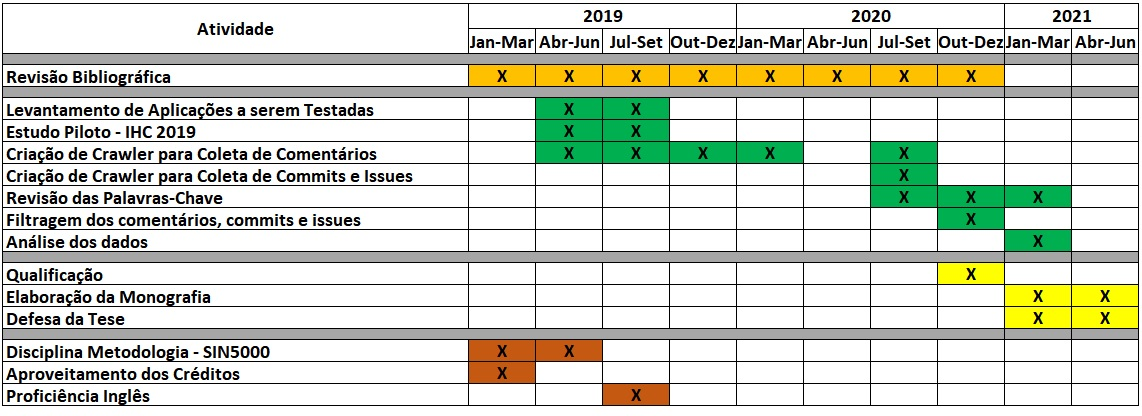
\includegraphics[scale=0.55]{imagens/Cronograma-v1.jpg}
	\caption{Cronograma - Imagem}
	\label{fig:cronograma}
\end{figure}

%%%%%%%%%%%%%%%%%%%%%%%%%%%
%%Tabela 1 - 10 trimestres%
%%%%%%%%%%%%%%%%%%%%%%%%%%%

********

tabela 1

********

\begin{table}[htbp]
	\centering
	\caption{Cronograma - tabela teste apenas - modelo PPGSI}
	\begin{tabular}{p{1in} p{1in} p{1in} p{1in} } \hline
		
		Atividade														& Jan-Mar	& Cabeçalho 3	& Cabeçalho 4 \\ \hline
		Revisão Bibliográfica											& número & número	& número \\ 
		Levantamento de Aplicações a serem Testadas (Acessibilidade)	& número & número	& número \\ 
		Texto	& número & número	& número \\ 
		Texto	& número & número	& número \\ 
		Texto	& número & número	& número \\ \hline
		
	\end{tabular}
	\label{tab:cronogramappgsi}
	\source{Marcelo Fantinato, 2015}
\end{table}


*******************************************

tabela 2 - não contem os trimestres de 2021

*******************************************


\begin{table}[htbp]
	\centering
	\caption{Cronograma 2019 / 2020}
	\label{tab:Cronograma}
	\begin{tabular}{p{3.40in} p{0.20in} p{0.20in} p{0.20in} p{0.20in} p{0.20in} p{0.20in} p{0.20in} p{0.20in}} \hline
		%	\begin{tabular}{lcccccccc}
		\textbf{Atividade}							& Jan Mar & Abr Jun & Jul Set & Out Dez & Jan Mar & Abr Jun & Jul Set & Out Dez \\ \hline
		Revisão Bibliográfica						& X		  & X 	 	& X		  & X  		& X  	  & X  		&         & 	    \\ 
		Levantamento de Aplicações a serem Testadas	& 		  & X	    & X		  &    		&  		  &  	    & 		  & 	    \\ 
		Teste de Falhas nas Aplicações	  			&  		  & 	    & X		  & X		&    	  &  	    &  	      & 		\\ 
		Criação de Crawler - Coleta de Comentários	&  		  & X       & X		  & X		&    	  &  	    &  	      & 		\\ 
		Identificação Parceria - Execução de Testes	&  		  & 	    & X		  & X		&    	  &  	    &  	      & 		\\ 
		Testes Utilizando PLN sobre Dados Coletados &  		  & 	    & X		  & X		& X  	  &  	    &  	      & 		\\
		Inclusão de Comentários para Aplicações		&  		  & 	    &  		  & X		& X  	  & X	    &  	      & 		\\
		Análise das Ações dos Desenvolvedores		&  		  & 	    &  		  &  		&    	  & X	    & X	      & 		\\ \hline
		Qualificação								&  		  & 	    &  		  &  		& X  	  &  	    &  	      & 		\\
		Elaboração da Monografia					&  		  & 	    &  		  &  		& X  	  & X	    & X	      & 		\\
		Defesa da Tese								&  		  & 	    &  		  &  		&    	  &  	    & X	      & X   	\\ \hline
		%Disciplina Metodologia - SIN5000			& X		  & X       &  		  &  		&    	  &  	    &  	      & 		\\
		Proficiência Inglês							&  		  & 	    & X		  & X		&    	  &  	    &  	      & 		\\
	\end{tabular}
\end{table}


*******************

tabela 3 - 30 meses

*******************



%%%%%%%%%%%%%%%%%%%%%%
%%Tabela 2 - 30 meses%
%%%%%%%%%%%%%%%%%%%%%%

\begin{table*}[!htb]
	\centering
	\caption{Cronograma - tabela teste apenas - versão 2}
	\label{tab:cronograma}
	\resizebox{\textwidth}{!}{ % abre resizebox, setar tabela da largura da página.
		\begin{tabular}{lcccccccccccccccccccccccccccccccc}
		\hline
		Atividade             							& 1 & 2 & 3 & 4 & 5 & 6 & 7 & 8 & 9 & 10 & 11 & 12 & 11 & 12 & 13 & 14 & 15 & 16 & 17 & 18 & 19 & 20 & 21 & 22 & 23 & 24 & 25 & 26 & 27 & 28 & 29 & 30 \\
		\hline
		Levantamento
		                      							&   &   &   &   &   &   &   &   &   &    &    &    &    &    &    &    &    &    &    &    &    &    &    &    &    &    &    &    &    &    &    &    \\
		Crawler Comentários
		                      							&   &   &   &   &   &   &   &   &   &    &    &    &    &    &    &    &    &    &    &    &    &    &    &    &    &    &    &    &    &    &    &    \\
		Estudo Piloto
		                      							&   &   &   &   &   &   &   &   &   &    &    &    &    &    &    &    &    &    &    &    &    &    &    &    &    &    &    &    &    &    &    &    \\
		Crawler Commits
														&   &   &   &   &   &   &   &   &   &    &    &    &    &    &    &    &    &    &    &    &    &    &    &    &    &    &    &    &    &    &    &    \\
		Crawler Issues
														&   &   &   &   &   &   &   &   &   &    &    &    &    &    &    &    &    &    &    &    &    &    &    &    &    &    &    &    &    &    &    &    \\
		\end{tabular}
	}
\end{table*}


\section{Contribuições}
As principais contribuições esperadas desta pesquisa são as evidências de que não só as aplicações móveis são pouco acessíveis, mas que também os requisitos relacionados à acessibilidade digital raramente são abordados durante a evolução de uma aplicação móvel.
Os resultados desta pesquisa podem contribuir com os estudos relacionados à acessibilidade digital em aplicações móveis e fomentar pesquisas e ações voltadas à conscientização e treinamento de desenvolvedores, e igualmente a criação de novos recursos para
a implementação e avaliação de acessibilidade digital.
Como contribuições adicionais entregues, podemos citar:

\begin{itemize}
	\item Conjunto de dados de comentários, \textit{commits} e \textit{issues} para posteriores estudos relacionados;
	\item Evolução dos conjuntos de palavras-chave relacionadas à acessibilidade, expandindo o mesmo para os padrões W3C e eMAG;
	\item Código fonte em Python que permita realizar a obtenção de comentários do \textit{Google Play Store}, dos \textit{commits} e \textit{issues} cadastrados no Github.
\end{itemize}



%3.1
%Descrição mais detalhada do que iremos fazer
%1 - pequisa introdução retomando o assunto: visto que os comentários são interessantes para os desenvolvedores, tem muitas informações para eles melhorarem, os motivam e que as aplicações têm pouca acessibilidade, queremos verificar se as pessoas enviam os comentário
%2 - queremos investigar se as pessoas comentam sobre acessibilidade dos repositórios
%3 - vamos detalhar nosso estudo para chegar a esta conclusão
%4 - estudo bibliográfico:
%estudar os guias de acessibilidade
%selecionar os aplicativos que serão analisados
%introdução
%metodologia
%selecionar os apps
%coletar os comentários
%filtrar os comentários
%keywords
%análise manual
%analisar comentários
%usar estatísticas: porquê? o que queremos com elas?
%porcentagem de comentários que envolvem acessibilidade
%porcentagens: basicamente aquilo que já está no artigo referente
%inserir gráficos, como no artigo
%PLN: por que utilizar PLN? Precisamos pensar o motivo
%Usos para PLN: dividir em tópicos, análise de sentimentos, neste sentido, podemos citar o artigo do Panichella
%Seria interessante fazermos uma análise temporal? Comentários ao longo do tempo. Analisar 3 meses seguidos? Comparar com as quantidades de comentários levantados no passado.
%olhar os dados e pensar
%Como estamos fazendo um estudo exploratório, não teríamos hipóteses a serem citadas
%O que queremos com todo este estudo: mostrar um panorama geral sobre isso tudo e tirar uma conclusão se isso é bastante, se é pouco


%3.2
%Citar as atividades já realizadas
%Descrever que já fizemos um estudo piloto motivacional: IHC2019
%descrever sucintamente, fazendo uma referência para o artigo

%3.3
%Cronograma
%listar as atividades, que estão relacionadas com tudo, incluindo o estudo piloto, colocando por mês ou bimestre, desde quando entrei como regular
%parecido com o que foi apresentado no ppt, quebrando um pouco mais do que por trimestre
%fizemos tudo isso, mas o quê queremos mais? analisamos poucos aplicativos, apenas 700, podemos ampliar este número de apps. Depois do estudo piloto aprendemos como fazer, agora queremos repetir para um número maior de aplicativos
%temos 2 opções: falar que vamos fazer novas análises, não feitas ainda no artigo, ou então vamos aprofundar mais as análises já feitas no artigo
%conclusão: tudo isso já fiz, mas falta esta parte ainda
%opção 1: melhorar o artigo fazendo estas análises, e daí termina o mestrado
%opção 2: ter uma outra estratégia, como por exemplo pegar os top 20 de cada categoria, pegar os tops pode me dar um resultado enviezado, já que os tops têm altos valores aportados (recursos) e por isso podem ter um retorno bom dos comentários. Precisamos saber o caso normal dos desenvolvedores
%fazer análises comparativas dos tops, aliatoriamente com alguns do meio, outros menos baixados, podemos identificar diferenças por serem tops, ou até mesmo não encontrar diferenças

%entrar na estratégia: quais serão as seleções que serão feitas, no estudo piloto tem descrito a estratégia que foi utilizada no artigo: pegou o que estava no github, aqueles que estavam no F-Droid, e então obteve os comentários. Até a qualificação foram feitos todos os itens, depois da qualificação temos novamente os passos, agora seguindo a estratégia que pretendemos utilizar

%importante: no estudo piloto tivemos uma análise manual sobre 5000 comentários. Podemos extrapolar as interpretações sobre as palavras chaves em todos os comentários que identificarmos, já que os volumes possivelmente serão maiores. mas devemos perder muito com esta extrapolação.
%outra opção seria a utilização de PLN para saber, mas precisaríamos validar com a Sarajane ou com o Ivandré. O estudo piloto também pode direcionar a exclusão de falsos positivos (ex: palavra (header). O estudo piloto serviu para identificarmos falsos positivos, principais keywords, montar uma estatística

%e no fim as considerações finais, retomar o que foi já feito. Muito do que está no artigo serve e me guiará no que deve ser feito.


\chapter{Atividades já realizadas}
\label{chap:atividades}
Este capítulo apresenta um estudo exploratório realizado com o objetivo de verificar a viabilidade e aperfeiçoar a proposta com base nas descobertas e desafios enfrentados durante o processo. Destaca-se que este estudo teve o foco apenas na análise das avaliações de acessibilidade e não explorou as sugestões de modificações e as alterações realizadas no código das aplicações. 


Todas as decisões de projeto e metodologia adotada estão em conformidade com o que foi descrito no Capítulo~\ref{chap:proposta}.
Além disso, também são descritas as atividades já realizadas do cronograma proposto.

\section{Questões de pesquisa}

As seguintes questões de pesquisa foram definidas para este estudo exploratório:
\begin{itemize}
 \item RQ1 - Quantas avaliações de usuário são relacionadas a acessibilidade e qual é a sua distribuição? 
 \item RQ2 - Qual é a diversidade de tópicos de acessibilidade abordados nas avaliações dos usuários?
 \item RQ3 - Quais são as notas associadas às avaliações que abordam aspectos de acessibilidade?  
\end{itemize}

\section{Seleção de aplicativos móveis}

Os critérios de seleção dos aplicativos para este estudo seguem os critérios definidos na Seção~\ref{sec:selecao}. Portanto, foram selecionadas aplicações da plataforma Android que satisfaziam as seguintes condições: estavam disponíveis na Google Play Store e o código-fonte estava armazenado em um repositório público da plataforma GitHub. Ao todo, apenas 701 aplicativos dentre os mais de 2000  indexados no FDroid\footnote{Dados de julho/2019} satisfizeram esses critérios.

A Tabela~\ref{tab:summarygps} mostra a distribuição de alguns atributos dos aplicativos selecionados por meio de estatística descritiva utilizando o resumo dos cinco números (mínimo amostral, quartil inferior, 
mediana, quartil superior, máximo amostral), a média e o desvio padrão. 
A maioria dos aplicativos tem até 9 atividades, mas há aplicativos muito maiores, como o ``Slide for Reddit'', por exemplo, que possui 91 atividades.

\begin{table}[htb]
%\setlength{\tabcolsep}{0pt}

\centering
\caption{Statistics on the Google Play Store sample}
\small
\label{tab:summarygps}
\begin{tabular}{lrrrrr}
\hline
             & Atividades & Nota & Avaliações     & Instalações  & Comentários \\
\hline
Mínimo          & 1          & 0     & 0            & 0         & 0       \\
Quartil Inferior           & 2          & 4           & 50    & 1K      & 4       \\
Mediana       & 5          & 4.3   & 130         & 10K     & 22      \\
Quartil Superior          & 9          & 4.6   & 836        & 50K     & 145     \\
Máximo          & 92         & 5     & 3.6M    & 100M & 4480    \\
Média         & 8.16       & 4.16  & 12.4K     & 550K+    & 305.4   \\
Desvio Padrão        & 10.5       & 0.79  & 151.6K  & 5.7M   & 840.8  \\
\hline
\end{tabular}
\end{table}

A maioria dos aplicativos possui uma boa nota e a maioria foi avaliada por até 836 usuários. O número de avaliações apresentado na tabela é diferente do número de comentários, pois quando um usuário faz uma avaliação ele é obrigado a atribuir uma nota, mas não é obrigado a inserir um comentário. Existem aplicativos que possuem um número muito alto de avaliações, como o Telegram, que possui 3,6 milhões de avaliações. O Telegram também é o aplicativo mais instalado (100 milhoes de istalações).
Por outro lado, o número de comentários não é muito alto, pois a maioria dos aplicativos recebeu até no máxmio 145 comentários em suas avaliações. O número máximo de revisões desta amostra é de 4480 em razão das limitações da API utilizada. Esta limitação não teve muito impacto neste estudo exploratório porque apenas 15 aplicativos (2\%) possuem mais de 4480 avaliações registradas na Google Play Store. 
Para as novas coletas de avaliações serão avaliadas outras alternativas para que não haja limite no número de avaliações retornadas pela API. 


\section{Extração e seleção das avaliações}
\label{sec:extracaoselecao}

Uma aplicação escrita na linguagem Python foi escrita para consumir os dados da Google Play Store utilizando a API \emph{google-play-api}\footnote{https://github.com/facundoolano/google-play-api}. Como mencionado anteriormente, na versão utilizada, esta API só permite o retorno de no máximo 4480 avaliações de cada aplicativo. Além disso, só foram recuperadas avaliações escritas em inglês, que é o idioma padrão definido pela API.


A seleção das avaliações que possivelmente estão relacionadas a algum aspecto de acessibilidade da aplicação foi feita por meio da utilização de palavras-chave aplicadas aos comentários dos usuários. 
Para isso, um conjunto de palavras-chave foi definido com base nas diretrizes de acessibilidade da BBC~\cite{bbc}. Este guia de acessibilidade possui 54 recomendações que são classificadas em onze diferentes categorias: áudio e vídeo (5); design (12); editorial (3); foco (6); formulários (6); imagens (2); links (3); notificações (4); scripts e conteúdo dinâmico (4); estrutura (4); e texto equivalente (5). 
Este padrão foi selecionado porque ele tem o foco em aplicações móveis e possui exemplos de implementação e de teste de cada recomendação, o que permite compreender melhor os tipos de problemas de acessibilidade tratados no guia. 

Foram definidas 213 palavras-chave com base na análise de cada recomendação do guia. 
A Tabela~{tab:keywords} mostra exemplos das palalavras-chave utilizadas.
Note que foram utilizadas variantes das palavras (exemplo: \textit{cannot see} e \textit{can't see}, ou \textit{color} e \textit{colour}, ou \textit{impaired} e \textit{impairement}) para garantir que nenhuma avaliação relevante fosse excluída. Infelizmente, não é possível capturar casos em que as palavras foram escritas com a grafia errada. A lista completa das palavras-chave podem ser vistas em um repositório criado para armazenar dos dados deste estudo\footnote{https://github.com/marceloeler/data-ihc2019}.


\begin{table}[!htb]
\small
\caption{Exemplos de palavras-chave utilizadas para selecionar avaliações relacionadas à acessibilidade das aplicações}
\label{tab:keywords}
\begin{tabular}{|l|l|}
\hline
Categorias & Palavras-chave \\
\hline
Gerais                    & accessibility, disability, screen reader, Talkback, operable, impaired, 
\\& impairment                                               \\

\hline
Áudio/Vídeo             & subtitle, sign language, audio description,
 transcript, autoplay, mute, \\& volume                                                 \\

\hline
Design                      & contrast, background color, blind, flicker,
 visual cue, touch size, \\&overlap, font size, 
 dark/light mode, eyestrain, seizure, can't see \\

\hline
Editorial                   & consist. label, language, visual/audio cue                                                                \\

\hline
Foco                       & focusable, control focus, keyboard trap, 
 focus order, navigable                        \\

\hline
Formulários                       & unique label, missing label, content description,
 input type, \\& input format, focusable                                                                        \\

\hline
Imagens                      & image of text, hidden text, text alternative,
background image                                                                                               \\

\hline
Links                       & link description, unique desc., duplicate
link, alternative format \\

\hline
Notificações               & inclusive, haptic, vibration, feedback, alert 
 dialog, understandable, \\& unfamiliar                                                                             \\

\hline
Conteúdo dinâmico & animated content, page refresh, automatic  
refresh, timeout,  adaptable, \\&input sign                                                               \\

\hline
Estrutura                   & page title, screen title, heading, header                                                                                                         \\
\hline
Texto equivalente             & alternative text, non-visual, blind, screen reader, content description  \\
\hline
\end{tabular}
\end{table}

O uso de palavras-chave pode trazer muitos falsos positivos, uma vez que várias palavras utilizadas podem ter conotações diferentes em diferentes contextos. Por isso foi realizada uma análise manual de todas as avaliações que possuíam pelo menos uma palavra-chave definida. Neste estudo, apenas uma pessoa fez a análise manual das avaliações. Além disso, as avaliações não selecionadas por palavras-chave não foram analisadas para saber se alguma delas não foi selecionada pela ausência de alguma palavra-chave relevante e que não foi utilizada. Durante a análise manual, as avaliações confirmadas também foram classificadas em: 
requisições, quando o usuário reporta algum problema de acessibilidade ou solicita alguma modificação ou adição para tornar a aplicação mais acessível;
ou elogios, quando o usuário parabeniza o aplicativo pelo seu nível de acessibilidade.


\section{Análise dos resultados}

As avaliações selecionadas com base nas palavras-chave e na validação manual foram analisadas para responder as questões de pesquisa propostas no estudo exploratório. A seguir as respostas às questões de pesquisa são apresentadas em detalhes. 

 
\textbf{RQ1 - Quantas avaliações de usuário são relacionadas a acessibilidade e qual é a sua distribuição? }

No total, foram extraídas 214.053 avaliações completas (com nota e comentário) dos 701 aplicativos da amostra. 
Dessas avaliações, apenas 5.076 foram pré-selecionadas por meio das palavras-chave. 
Após a análise manual, o número de avaliações relacionadas à acessibilidade das aplicações foi reduzido para 2.663, o que representa apenas 1.24\% de todas as avaliações completas extraídas.

As avaliações de acessibilidade não estão igualmente distribuídas entre os aplicativos da amostra.
Só 40\% dos aplicativos (276) possuem pelo menos uma avaliação relacionada a acessibilidade.
É importante ressaltar que 92\% (197.419) de todas as avaliações extraídas foram realizadas para esses 276 aplicativos, indicando que quanto menos avaliações, menos as chances de haver uma avaliação de acessibilidade. 
De fato, a correlação de Spearman calculada entre o número de avaliações e o número de avaliações de acessibilidade é de 0.73, o que representa uma forte correlação.

As avaliações de acessibilidade não estão distribuídas igualmente entre os 276 aplicativos.
Quase 65\% das avaliações de acessibilidade (1.745) estão concentradas em apenas 35 aplicativos. 
Dentre esses 35 aplicativos, três possuem mais de 100 avaliações de acessibilidade enquanto os demais tem entre 19 e 79 avaliações cada. 
A Figura~\ref{fig:distributionreviewsapp} mostra a distribuição de avaliações de acessibilidade entre os aplicativos da amostra, com exceção dos 35 aplicativos mencionados anteriormente.
É possível perceber que a grande maioria de aplicativos tem menos do que nove avaliações de acessibilidade enquanto cerca de metade da amostra tem até três avaliações do tipo.


\begin{figure}[!htb]
\centering
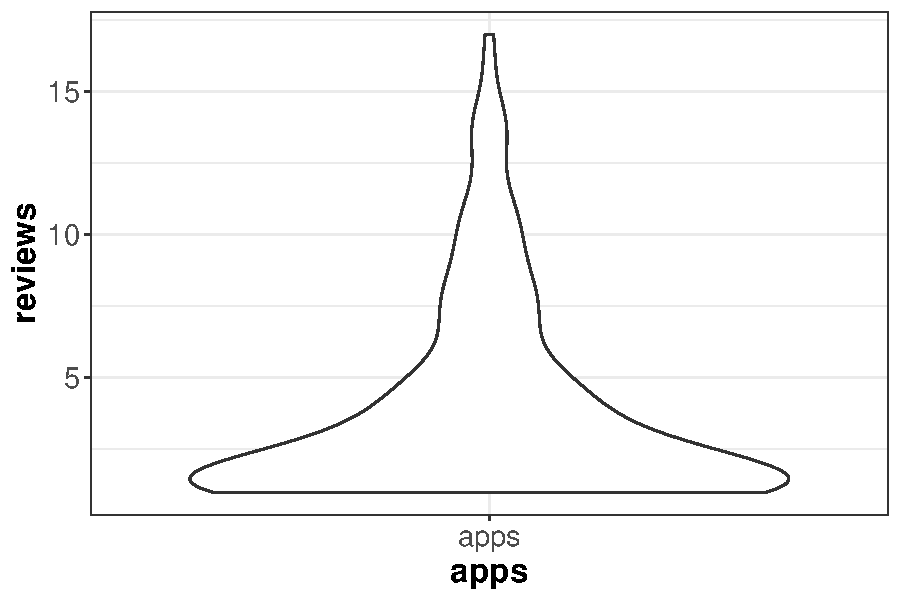
\includegraphics[scale=0.80]{imagens/distribution-accreviews-no-outlier-violin.pdf}
\caption{Distribuição das avaliações de acessibilidade entre os aplicativos da amostra}
\label{fig:distributionreviewsapp}
\end{figure}


A Figura~\ref{fig:distribution-proportion} mostra a distribuição da proporção entre as avaliações de acessibilidade e o número total de avaliações completas de cada aplicativo.
No geral, as avaliações de acessibilidade representam menos de 4\% de todas as reviões feitas para cada aplicativo. Para metade dos aplicativos, elas representam menos de 1.5\%.
Para uma pequena proporção de aplicativos, as avaliações de acessibilidade representam entre 4\% e 9\% das avaliações recebidas. Existem alguns aplicativos para os quais essa proporção varia entre 10\% e 16\%.
Há alguns casos em que o número de avaliações completas é tão pequeno que uma simples avaliação de acessibilidade representa uma grande proporção, como é o caso do aplicativo MuPDF mini, Booky McBookface, e GameDealz, cujas proporções são de 50\% (1/2), 40\% (2/5) e 33\% (1/3), respectivamente. 
\newline 

 \begin{figure}[!htb]
 \centering
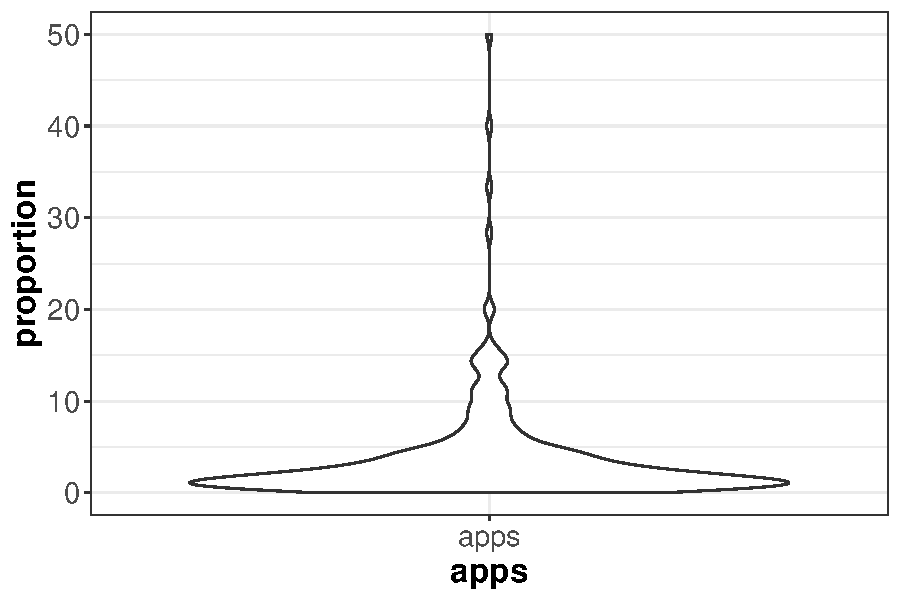
\includegraphics[scale=0.8]{imagens/distribution-proportion-accreviews}
\caption{Distribuição da proporção entre avaliações de acessibilidade e o total de avaliações de cada aplicativo}
\label{fig:distribution-proportion}
\end{figure}


\textbf{RQ2 - Qual é a diversidade de tópicos de acessibilidade abordados nas avaliações dos usuários?}

O objetivo desta questão de pesquisa é entender se os usuários abordam diferentes problemas de acessibilidade em suas avaliações ou se a maioria das avaliações tratam de um conjunto restrito de problemas. 
A Tabela~\ref{tab:keywords-reviews} mostra o número de avaliações de acessibilidade e aplicativos associado a cada palavra-chave utilizada para selecionar as avaliações. 
Nesta tabela só estão apresentadas as palavras-chave para as quais pelo menos uma avaliação estava associada. 

\begin{table*}[!htb]
\centering
\small
\setlength{\tabcolsep}{3pt}
\caption{Número de avaliações e aplicativos por palavra-chave}
\label{tab:keywords-reviews}
\begin{tabular}{lrr||lrr||lrr}
\hline
palavra          & avals. & apps & palavra          & avals. & apps &  palavra            & avals. & apps \\
\hline
dark mode        & 645     & 128  & metadata         & 20      & 12   & grouped            & 3       & 3    \\
zoom             & 491     & 80   & too bright       & 20      & 8    & seizures           & 3       & 1    \\
customization    & 309     & 50   & haptic           & 16      & 10   & select language    & 3       & 3    \\
font size        & 214     & 74   & scaling          & 16      & 11   & understandable     & 3       & 3    \\
volume           & 146     & 40   & control key      & 15      & 5    & vibration feedback & 3       & 3    \\
cannot see       & 128     & 57   & voice command    & 14      & 10   & actionable         & 2       & 1    \\
accessibility    & 74      & 44   & text-to-speech   & 13      & 9    & audio cue          & 2       & 2    \\
readable         & 72      & 47   & eyestrain        & 12      & 9    & missing label      & 2       & 2    \\
change font      & 68      & 44   & strain           & 12      & 9    & navigable          & 2       & 2    \\
hard to see      & 58      & 41   & backgrd. image & 11      & 8    & verbose            & 2       & 2    \\
backgrd. color   & 50      & 30   & screen reader    & 11      & 10   & captcha            & 2       & 2    \\
light mode       & 42      & 27   & change language  & 10      & 8    & audio description  & 1       & 1    \\
mute             & 42      & 25   & small widget     & 10      & 9    & container          & 1       & 1    \\
contrast         & 40      & 31   & stop button      & 10      & 5    & distinguishable    & 1       & 1    \\
subtitle         & 40      & 7    & impaired         & 9       & 9    & input type         & 1       & 1    \\
adjustable       & 34      & 23   & text reflow      & 9       & 3    & keyboard language  & 1       & 1    \\
blind            & 31      & 24   & timeout          & 9       & 7    & page refresh       & 1       & 1    \\
header           & 31      & 22   & consistency      & 7       & 7    & page title         & 1       & 1    \\
overlap          & 31      & 25   & epilepsy         & 7       & 1    & sign language      & 1       & 1    \\
pause button     & 27      & 17   & assistance       & 6       & 5    & svg image          & 1       & 1    \\
flicker          & 26      & 19   & colour coding    & 5       & 5    & switch device      & 1       & 1    \\
spacing          & 26      & 17   & transcript       & 5       & 5    & touch target       & 1       & 1    \\
migraine         & 25      & 3    & default language & 4       & 4    & adjust size        & 1       & 1    \\
input method     & 23      & 11   & older device     & 4       & 3    & adjust colour      & 1       & 1    \\
autoplay         & 21      & 17   & visual cue       & 4       & 4    &                    &         &     \\
\hline
\end{tabular}
\end{table*}

Claramente, as avaliações de acessibilidade estão concentradas em um pequeno conjunto de palavras-chave. Seis das palavras-chave mais populares são mencionadas em mais de 100 avaliações de diferentes aplicativos. Por exemplo, a palavra-chave \textit{dark mode} aparece em 628 avaliações de 128 aplicativos distintos, o que representa quase metade da amostra de aplicativos.

Como várias palavras-chave podem estar relacionadas a uma mesma diretriz ou princípio de acessibilidade (exemplo: \textit{dark mode}, \textit{night mode} e \textit{black mode}), 
as palavras-chave e as respectivas quantidades de avaliações foram agrupadas por tópicos (diretrizes, princípios ou temas) específicos de acessibilidade para facilitar a análise da diversidade de características abordadas.

A Tabela~\ref{tab:group-keywords} mostra, para cada tópico de acessibilidade (Coluna 1), o número de avaliações distintas (Coluna 2), a proporção das avaliações em relação às avaliações de acessibilidade (Coluna 3), o número de aplicativos distintos que tiveram uma avaliação relacionada (Coluna 4), e a proporção de aplicativos em relação aos aplicativos que possuem pelo menos uma avaliação (Coluna 5).
As diretrizes gerais da BBC não foram utilizadas para a organização dos tópicos apresentados na tabela porque eles são muito gerais e podem englobar muitas palavras-chave ao mesmo tempo.

\begin{table}[]
\centering
\caption{Distribuição de avaliações de acessibilidade e aplicativos por tópico de acessibilidade}
\label{tab:group-keywords}
\begin{tabular}{lrrrr}
\hline
Tópico         & Avals. & \% (Avals.) & Apps & \% (Apps) \\
\hline
Theme/Mode    & 726     & 27\%     & 144  & 52\%  \\
Zoom          & 506     & 19,0\%     & 83   & 30,1\%  \\
Customization & 351     & 13\%     & 63   & 23\%  \\
Media         & 309     & 11,6\%     & 82   & 29,7\%  \\
Font          & 249     & 9,4\%      & 83   & 30,1\%  \\
Contrast      & 218     & 8\%        & 91  & 33\%  \\
Impairment    & 135     & 5,1\%      & 70   & 25,4\%  \\
Flickering    & 87      & 3,3\%      & 31   & 11,2\%  \\
Accessibility & 74      & 2,8\%      & 44   & 15,9\%  \\
Size          & 66      & 2,5\%      & 45   & 16,3\%  \\
Input alternatives        & 54      & 2,0\%      & 25   & 9,1\%   \\
Feedback      & 19      & 0,7\%      & 11   & 4,0\%   \\
Language      & 15      & 0,6\%      & 11   & 4,0\%  \\
\hline
\end{tabular}
\end{table}

O tópico \textit{Theme/Mode} é o mais popular entre as avaliações uma vez que 27\% das avaliações de acessibilidade estão relacionadas a este tópico, e quase metade das aplicações tem este tipo de avaliação. 
Este tópico agrega todas as avaliações que mencionam modos de cores e temas das interfaces dos aplicativos. 
O segundo tópico mais popular é o relacionado a funcionalidades de \textit{zoom} (19\% das revisões de acessibilidade e 30\% das aplicações).
O terceiro tópico mais popular está relacionado à personalização do aplicativo, representando 13\% das revisões e relacionados a 23\% dos aplicativos. 
Diversos outros tópicos estão presentes em um número menor de avaliações de acessibilidade, mas muitos deles estão relacionados com um grande número de aplicativos. 

Além da análise de todas as avaliações em conjunto, também foram realizadas análises das diversidades de tópicos de acessibilidade de cada aplicativo isoladamente. 
Figure~\ref{fig:distributiontopicsapps} mostra a distribuição de palavras-chave encontradas nas avaliações de acessibilidade de cada aplicativo (lado esquerdo). 
No geral, há pouca diversidade de palavras-chave nas avaliações de cada aplicativo analisado individualmente. 
A correlação de Spearman entre a diversidade de palavras-chave e o número de avaliações em cada aplicativo é de 0.93, o que indica que a diversidade aumenta conforme aumenta o número de avaliações.


 \begin{figure}[!htb]
 \centering
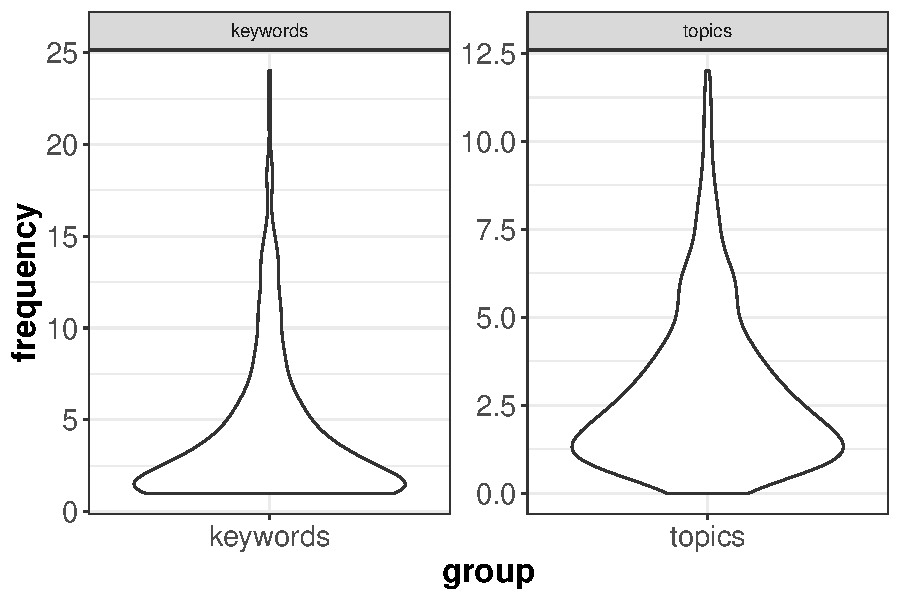
\includegraphics[scale=0.8]{imagens/distribution-topics-keywords.pdf}
\caption{Distribuição de tópicos de acessibilidade e palavras-chave nas avaliações de cada aplicativo}
\label{fig:distributiontopicsapps}
\end{figure}


Para a maioria dos aplicativos, as avaliações de acessibilidade estão relacionadas a no máximo seis palavras-chave. 
Para metade dos aplicativos, no máximo três palavras-chave são mencionadas. 
Poucos aplicativos tem avaliações que mencionam mais de 15 palavras-chave. 
Um dos aplicativos que foge ao padrão é o \textit{Cool Reader}, pois em suas avaliações foram encontradas 36 palavras-chave distintas. 


A diversidade de palavras-chave não é uma indicação de que diversos aspectos de acessibilidade são tratados uma vez que muitas delas estão relacionadas a um mesmo problema, e por isso uma análise por tópico deve ser realizada. 
A Tabela~\ref{fig:distributiontopicsapps} mostra a distribuição de tópicos de acessibilidade relacionados a cada avaliação de acessibilidade (lado direito). 
Note que as avaliações de acessibilidade para a maioria dos aplicativos estão concentradas em dois a quatro tópicos, enquanto alguns aplicativos possuem avaliações associadas a quase todos os tópicos abordados. 
O aplicativo \textit{Calculator}, por exemplo, tem avaliações de acessibilidade que abordam 12 tópicos de acessbilidade distintos. 
Embora a correlação de Spearman entre a diversidade de tópicos e o número de avaliações seja de 0.87, o que representa uma correlação forte, este aplicativo possui apenas 60 avaliações. \newline


\textbf{RQ3 - Quais são as notas associadas às avaliações que abordam aspectos de acessibilidade?}


Durante a validação manual (ver Seção~\ref{sec:extracaoselecao}), as avaliações foram classificadas entre requisições (76\%) ou elogios (24\%).
As 645 avaliações que elogiam a acessibilidade estão distribuídas por 110 aplicativos, enquanto as requisitções estão distribuídas por 262 aplicativos. 
Um dos propósitos desta questão de pesquisa é entender se os usuários dão uma nota boa para o aplicativo quanto fazem um elogio e uma nota ruim quanto fazem alguma requisição. 
A Figura~\ref{fig:reqcompscores} mostra a comparação das notas recebidas pelas avaliações classificadas nessas duas categorias. Aparentemente, não há nenhuma diferença significativa entre as notas atribuídas aos dois grupos.

 \begin{figure}[!htb]
 \centering
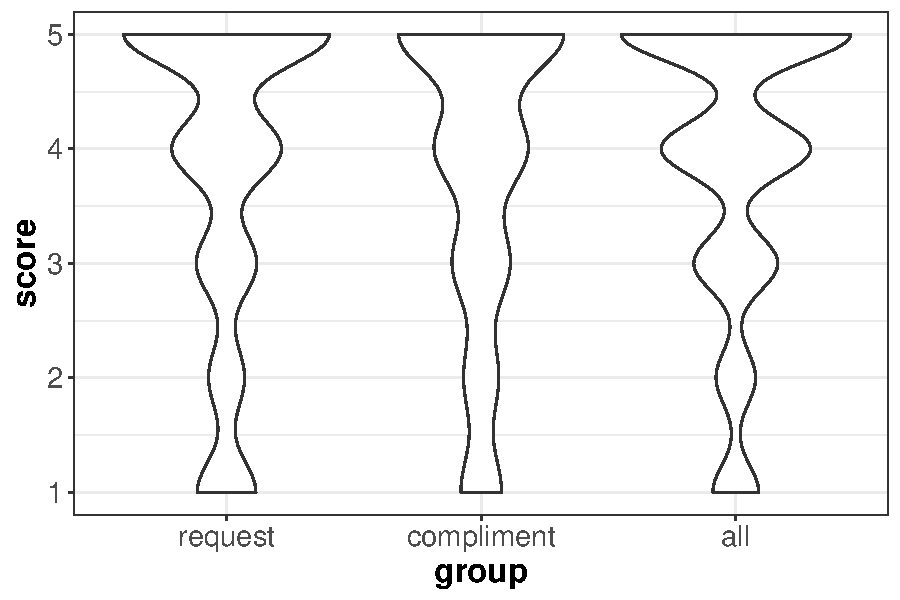
\includegraphics[scale=0.8]{imagens/scores-compliment-request.pdf}
\caption{Comparação entre as notas associadas a avaliações que contem requisições com as avaliações que contem elogios à acessibilidade dos aplicativos}
\label{fig:reqcompscores}
\end{figure}

Adicionalmente, deseja-se descobrir se avaliações associadas a diferentes palavras-chave ou tópicos de acessibilidade possuem notas maiores ou menores. 
A Figura~\ref{fig:scoresthemes} mostra as notas associadas a cada tópico de acessibilidade (ver~ \ref{tab:group-keywords}). 
Neste caso, nós só consideramos avaliações que contem requisições. 
Para alguns tópicos específicos, mesmo que haja requisição dos usuários para tornar as aplicações mais acessíveis, as notas são, em sua maioria, 4 ou 5 (exemplo: \textit{customization}, \textit{font}, \textit{media}, \textit{size} e \textit{theme}).
Para outros tópicos, entretanto, as notas estão concentradas em valores mais baixos, de 2 a 4 (exemplo: \textit{contrast}, \textit{flickering} e \textit{zoom}). 


 \begin{figure}[!htb]
 \centering
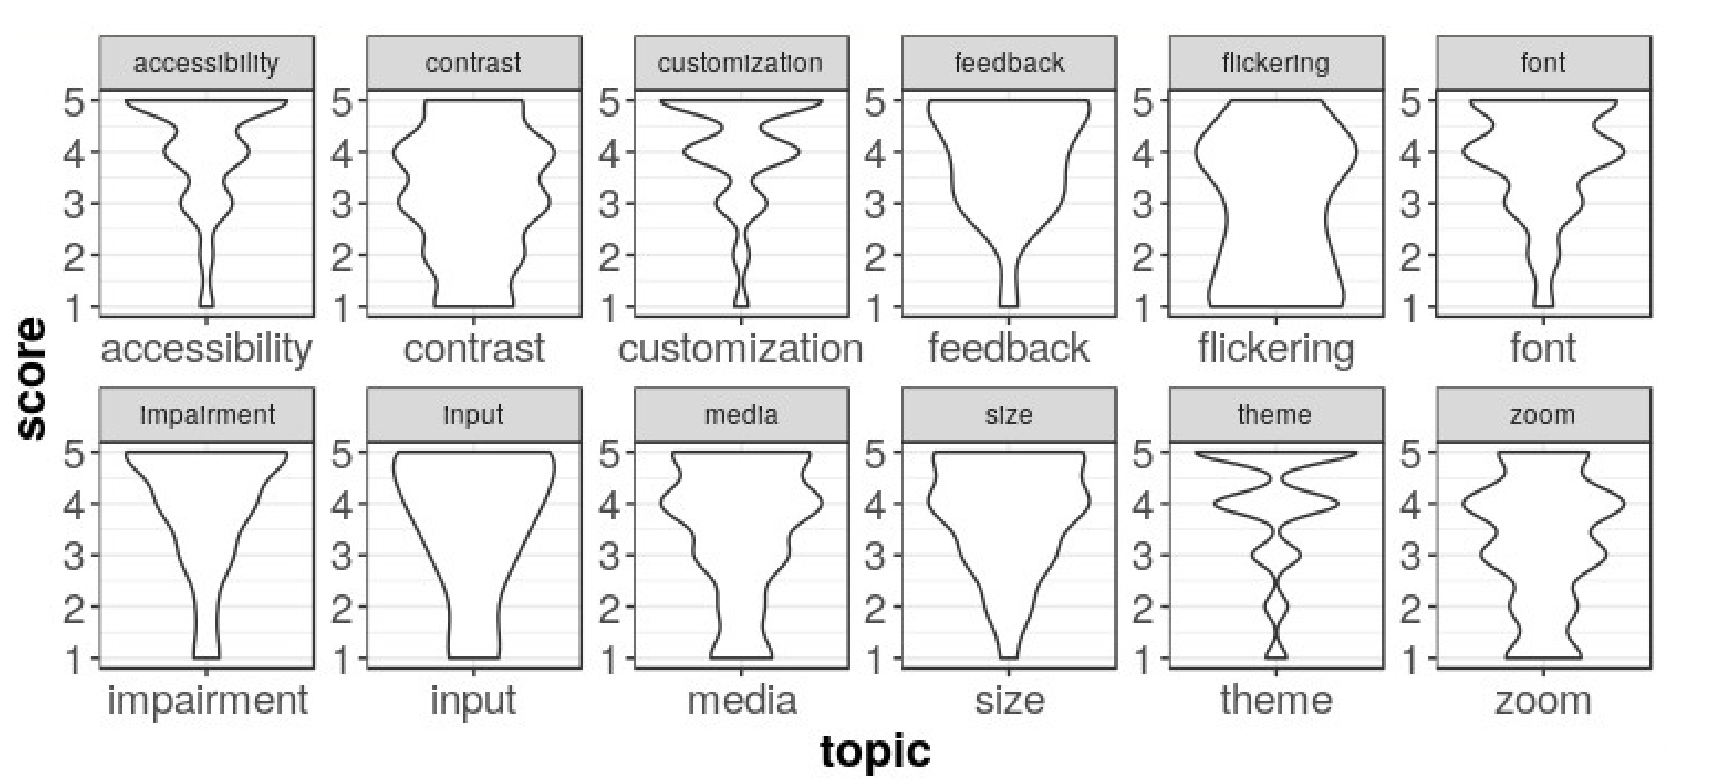
\includegraphics[scale=0.57]{imagens/score-themes-adapt.pdf}
\caption{Scores associated with the reviews that address an accessibility topic (cf. \autoref{tab:group-keywords})}
\label{fig:scoresthemes}
\end{figure}

A Figura~\ref{fig:scoreskeys} mostra as notas associadas a avaliações que contem algumas das  palavras-chave utilizadas neste estudo. 
Para algumas palavras-chave, as notas estão concentradas nos valores máximos (\textit{accessibility}, \textit{blind}, \textit{change font}, \textit{dark mode}, \textit{customization}, \textit{haptic}, etc).
Para outras palavras-chave, as notas são significativamente mais baixas (\textit{cannot see}, \textit{epilepsy}, \textit{flicker}, \textit{migraine}, \textit{readable}, \textit{text reflow} e \textit{too bright}). 

 \begin{figure}[!htb]
 \centering
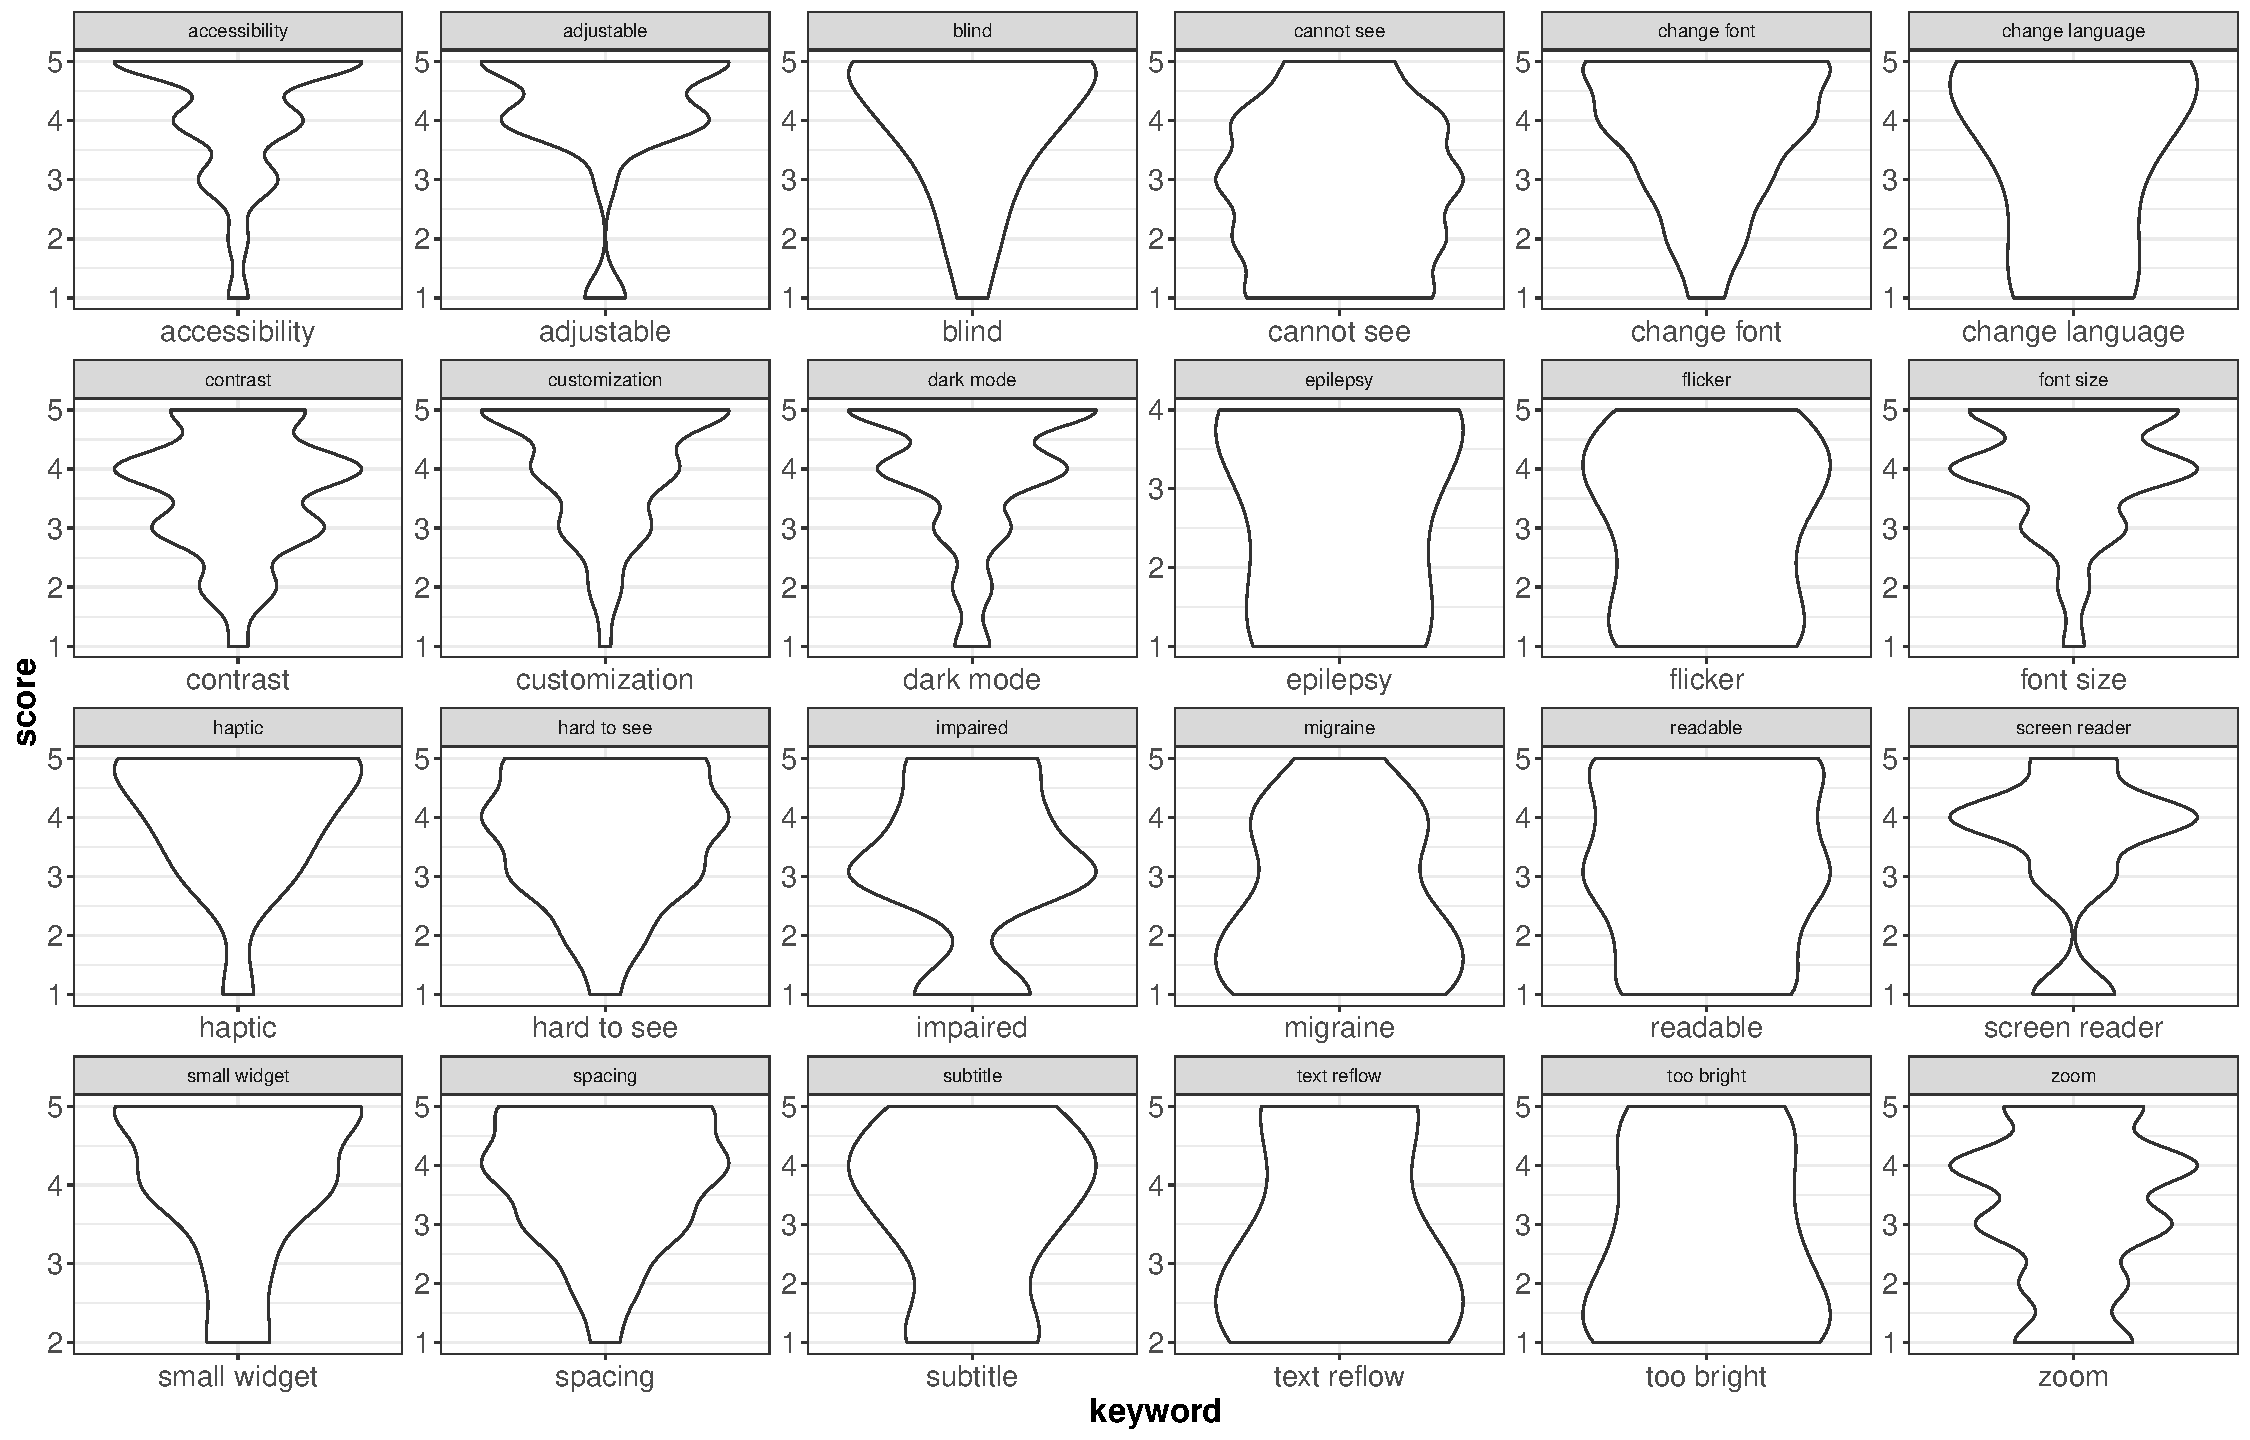
\includegraphics[scale=0.42]{imagens/keywords-scores.pdf}
\caption{Scores associated with the reviews that present a particular keyword}
\label{fig:scoreskeys}
\end{figure}

Aparentemente, os usuários só atribuem notas baixas aos aplicativos quando encontram problemas de acessibilidade que são barreiras para a utilização do aplicativo. 
Alguns exemplos de comentários de usuários encontrados nas avaliações que contem palavras-chave associadas a menores notas estão apresentados a seguir:
\begin{itemize}
 \item \textit{``Very little contrast. Bad for old eyes.''}
 \item \textit{``Wish it also handled older open doc formats - and that it would reflow text on zoom''}
 \item \textit{`` The flashing backgrounds could trigger an epilepsy and migraine''}
 \item \textit{``It's ok but the editing icons come up in white over the image.. which obviously means if you have a white image you cannot see them. Seriously - how could a developer get something so obvious that wrong? ''}
 \item \textit{`` Widget Text color is black. Unreadable''}
 \item \textit{``Too bright now on this update now. Can you option to inverted color? (black instead of white). Going to have to uninstall. Sorry.''}  
\end{itemize}



\section{Discussão}

A maioria das avaliações de acessibilidade encontradas foram feitas por usuários que não necessariamente estavam tratando diretamente da acessibilidade da aplicação. Ainda que essas avaliações mencionem aspectos da aplicação que influenciam a sua acessibilidade, nem todas elas são requisições relacionadas a barreiras encontradas pelos usuários, mas solicitações para melhorar sua experiência de uso. 
Embora poucos usuários se identifiquem como pessoas com deficiência em suas avaliações, percebe-se que as requisições realizadas por eles são associadas a barreiras reais encontradas durante o uso da aplicação, acompanhadas de notas mais baixas dadas ao aplicativo. 

Em geral, pessoas com deficiência tendem a ser enfáticas sobre as barreiras que as impedem de usar plenamente a apliação. A seguir são apresentados alguns exemplos de comentários feitos por pessoas com deficiência:
\begin{itemize}
 \item \textit{``I am legally blind and use Voice Assistant. This app does not interface well with Voice Assistant. It jumps to reading the logo - when trying to get to next group or text to be read. Extremely frustrating! Please fix right away!''}
  \item \textit{``The layout of the app is miserable for those with visual impairments. Please rethink your layout for those who can't read the tiny clues (even on a tablet!)''}
  \item \textit{``Some buttons are unlabelled (I've figured out which ones are repeat and shuffle - I still don't think I know what some are). Also the sleep timer is half-way accessible - when I was using the slider to select the minutes it wouldn't read the amount of time I selected (might be the fault of the screen reader though - I'm using the Mobile Accessibility screen reader from Code Factory).''}
  \item \textit{``Hello. If this app become accessible to Talkback (android screen reader) I wish the best for you developers. Actually we blinds can use telegram only on ios because it is accessible with Voiceover (IOS screen reader). One of my friends needs it because he does not have money to buy an apple product but he has a cheap android device and he needs telegram on it because of their university channel on telegram. If this app becomes accessible I will rate it 5 or more!''}
  \item \textit{``What are you trying to do? Give someone who has epilepsy a seizure? I almost did. Thanks a lot, idiots''}  
\end{itemize}

A escassez e a homoneidade das avaliações de acessibilidade associadas às boas notas recebidas em geral pelos aplicativos parece indicar que ou os usuários com deficiência não utilizam essas aplicações ou eles tendem a realizar avaliações. 
Nos estudos ampliados que serão realizados com base neste estudo exploratório, pretende-se fazer análise separadas de avaliações que claramente foram escritas por pessoas com alguma deficiência ou que enfrentaram uma barreira real para a utilização da aplicação pela falta de acessibilidade. 

Por fim, considerando que as avaliações dos usuários são uma poderosa ferramenta para guiar a evolução de aplicações móveis~\cite{Iacob2014online,Panichella2015how,Palomba2018crowdsourcing}, 
esses resultados preliminares sugerem que isso não tem sido utilizado apropriadamente para pressionar desenvolvedores e organizações na melhoria da acessibilidade das aplicações.

\section{Publicações}

Os resultados deste estudo exploratório foram divulgados em artigo completo publicado na trilha principal do XVIII Simpósio Brasileiro sobre Fatores Humanos em Sistemas Computacionais (IHC 2019)~\cite{ihc2019}. Destaca-se que este artigo recebeu o prêmio de melhor artigo do IHC 2019. 

\section{Nova seleção de aplicativos}

\textbf{Se der tempo: } É preciso realizar novamente uma seleção de aplicativos (FDroid X GPS X GitHub). O número tente a ser maior porque já passou um ano. Fazer um resumo sobre as informações dos aplicativos.

\section{Novas extrações de avaliações de usuários}

\textbf{Se der tempo: } É preciso extrair as avaliações dos aplicativos selecionados anteriormente. Vamos ver se não existe mais aquela restrição dos 4480 reviews. Fazer um resumo dos números até aqui. 

\section{Extração de sugestões de mudanças e de alterações realizadas nos aplicativos}

\textbf{Se der tempo: } É preciso extrair as issues e commits dos repositórios dos aplicativos selecionados. Fazer um resumo dos números até aqui. 

Depois pensamos nas palavras-chave para selecionar tudo. Vamos primeiro extrair tudo o que der e depois pensar na seleção e rodar todo o estudo de novo com um conjunto ampliado. 




% ----------------------------------------------------------
% ELEMENTOS PÓS-TEXTUAIS
% ----------------------------------------------------------
\postextual
% ----------------------------------------------------------

% ----------------------------------------------------------
% Referências bibliográficas
% ----------------------------------------------------------
\bibliography{referencias}


\end{document}
